% -*- Mode:TeX -*-

%% IMPORTANT: The official thesis specifications are available at:
%%            http://libraries.mit.edu/archives/thesis-specs/
%%
%%            Please verify your thesis' formatting and copyright
%%            assignment before submission.  If you notice any
%%            discrepancies between these templates and the
%%            MIT Libraries' specs, please let us know
%%            by e-mailing thesis@mit.edu

%% The documentclass options along with the pagestyle can be used to generate
%% a technical report, a draft copy, or a regular thesis.  You may need to
%% re-specify the pagestyle after you \include  cover.tex.  For more
%% information, see the first few lines of mitthesis.cls.

%\documentclass[12pt,vi,twoside]{mitthesis}
%%
%%  If you want your thesis copyright to you instead of MIT, use the
%%  ``vi'' option, as above.
%%
%\documentclass[12pt,twoside,leftblank]{mitthesis}
%%
%% If you want blank pages before new chapters to be labelled ``This
%% Page Intentionally Left Blank'', use the ``leftblank'' option, as
%% above.

\documentclass[12pt,twoside,vi,leftblank]{mitthesis}
%% These have been added at the request of the MIT Libraries, because
%% some PDF conversions mess up the ligatures.  -LB, 1/22/2014
\usepackage{cmap}
\usepackage[T1]{fontenc}
\usepackage[final]{listings}
\usepackage{multicol}
\usepackage{graphicx}
\usepackage{caption}
\usepackage{amsmath}
\usepackage{array}
\usepackage[hyphens]{url}
\usepackage[hidelinks]{hyperref}

\usepackage[math]{cellspace}
\setlength\cellspacetoplimit{0.5em}
\setlength\cellspacebottomlimit{0.5em}

\pagestyle{plain}
\graphicspath{{../images/}}


\begin{document}

% -*-latex-*-
%
% For questions, comments, concerns or complaints:
% thesis@mit.edu
%
%
% $Log: cover.tex,v $
% Revision 1.8  2008/05/13 15:02:15  jdreed
% Degree month is June, not May.  Added note about prevdegrees.
% Arthur Smith's title updated
%
% Revision 1.7  2001/02/08 18:53:16  boojum
% changed some \newpages to \cleardoublepages
%
% Revision 1.6  1999/10/21 14:49:31  boojum
% changed comment referring to documentstyle
%
% Revision 1.5  1999/10/21 14:39:04  boojum
% *** empty log message ***
%
% Revision 1.4  1997/04/18  17:54:10  othomas
% added page numbers on abstract and cover, and made 1 abstract
% page the default rather than 2.  (anne hunter tells me this
% is the new institute standard.)
%
% Revision 1.4  1997/04/18  17:54:10  othomas
% added page numbers on abstract and cover, and made 1 abstract
% page the default rather than 2.  (anne hunter tells me this
% is the new institute standard.)
%
% Revision 1.3  93/05/17  17:06:29  starflt
% Added acknowledgements section (suggested by tompalka)
%
% Revision 1.2  92/04/22  13:13:13  epeisach
% Fixes for 1991 course 6 requirements
% Phrase "and to grant others the right to do so" has been added to
% permission clause
% Second copy of abstract is not counted as separate pages so numbering works
% out
%
% Revision 1.1  92/04/22  13:08:20  epeisach

% NOTE:
% These templates make an effort to conform to the MIT Thesis specifications,
% however the specifications can change.  We recommend that you verify the
% layout of your title page with your thesis advisor and/or the MIT
% Libraries before printing your final copy.
\title{Matching Startup Founders to Investors: \\ a Tool and a Study}

\author{Yasyf Mohamedali}
% If you wish to list your previous degrees on the cover page, use the
% previous degrees command:
%       \prevdegrees{A.A., Harvard University (1985)}
% You can use the \\ command to list multiple previous degrees
%       \prevdegrees{B.S., University of California (1978) \\
%                    S.M., Massachusetts Institute of Technology (1981)}
\department{Department of Electrical Engineering and Computer Science}

% If the thesis is for two degrees simultaneously, list them both
% separated by \and like this:
% \degree{Doctor of Philosophy \and Master of Science}
\degree{Master of Engineering in Electrical Engineering and Computer Science}

% As of the 2007-08 academic year, valid degree months are September,
% February, or June.  The default is June.
\degreemonth{June}
\degreeyear{2018}
\thesisdate{May 18, 2018}

%% By default, the thesis will be copyrighted to MIT.  If you need to copyright
%% the thesis to yourself, just specify the `vi' documentclass option.  If for
%% some reason you want to exactly specify the copyright notice text, you can
%% use the \copyrightnoticetext command.
\copyrightnoticetext{\copyright 2018 Copyright Massachusetts Institute of Technology. All rights reserved.}

% If there is more than one supervisor, use the \supervisor command
% once for each.
\supervisor{John V. Guttag}{Dugald C. Jackson Professor of Computer Science and Electrical Engineering}

\supervisor{Rei Wang}{Director of Dorm Room Fund, First Round Capital}

% This is the department committee chairman, not the thesis committee
% chairman.  You should replace this with your Department's Committee
% Chairman.
\chairman{Christopher J. Terman}{Chair, Master of Engineering Thesis Comittee}

% Make the titlepage based on the above information.  If you need
% something special and can't use the standard form, you can specify
% the exact text of the titlepage yourself.  Put it in a titlepage
% environment and leave blank lines where you want vertical space.
% The spaces will be adjusted to fill the entire page.  The dotted
% lines for the signatures are made with the \signature command.
\maketitle

% The abstractpage environment sets up everything on the page except
% the text itself.  The title and other header material are put at the
% top of the page, and the supervisors are listed at the bottom.  A
% new page is begun both before and after.  Of course, an abstract may
% be more than one page itself.  If you need more control over the
% format of the page, you can use the abstract environment, which puts
% the word "Abstract" at the beginning and single spaces its text.

%% You can either \input (*not* \include) your abstract file, or you can put
%% the text of the abstract directly between the \begin{abstractpage} and
%% \end{abstractpage} commands.

% First copy: start a new page, and save the page number.
\cleardoublepage
% Uncomment the next line if you do NOT want a page number on your
% abstract and acknowledgments pages.
% \pagestyle{empty}
\setcounter{savepage}{\thepage}
\begin{abstractpage}
% $Log: abstract.tex,v $
% Revision 1.1  93/05/14  14:56:25  starflt
% Initial revision
%
% Revision 1.1  90/05/04  10:41:01  lwvanels
% Initial revision
%
%
%% The text of your abstract and nothing else (other than comments) goes here.
%% It will be single-spaced and the rest of the text that is supposed to go on
%% the abstract page will be generated by the abstractpage environment.  This
%% file should be \input (not \include 'd) from cover.tex.
The process of matching startup founders with venture capital investors is a necessary first step for many modern technology companies, yet there have been few attempts to study the characteristics of the two parties and their interactions. Surprisingly little has been shown quantitatively about the process, and many of the common assumptions are based on anecdotal evidence. In this thesis, we aim to learn more about the matching component of the startup fundraising process. We begin with a tool (VCWiz), created from the current set of best-practices to help inexperienced founders navigate the founder-investor matching process. The goal of this tool is to increase efficiency and equitability, while collecting data to inform further studies. We use this data, combined with public data on venture investments in the USA, to draw conclusions about the characteristics of venture financing rounds. Finally, we explore the communication data contributed to the tool by founders who are actively fundraising, and use it to learn which social attributes are most beneficial for individuals to possess when soliciting investments.

\end{abstractpage}

% Additional copy: start a new page, and reset the page number.  This way,
% the second copy of the abstract is not counted as separate pages.
% Uncomment the next 6 lines if you need two copies of the abstract
% page.
% \setcounter{page}{\thesavepage}
% \begin{abstractpage}
% % $Log: abstract.tex,v $
% Revision 1.1  93/05/14  14:56:25  starflt
% Initial revision
%
% Revision 1.1  90/05/04  10:41:01  lwvanels
% Initial revision
%
%
%% The text of your abstract and nothing else (other than comments) goes here.
%% It will be single-spaced and the rest of the text that is supposed to go on
%% the abstract page will be generated by the abstractpage environment.  This
%% file should be \input (not \include 'd) from cover.tex.
The process of matching startup founders with venture capital investors is a necessary first step for many modern technology companies, yet there have been few attempts to study the characteristics of the two parties and their interactions. Surprisingly little has been shown quantitatively about the process, and many of the common assumptions are based on anecdotal evidence. In this thesis, we aim to learn more about the matching component of the startup fundraising process. We begin with a tool (VCWiz), created from the current set of best-practices to help inexperienced founders navigate the founder-investor matching process. The goal of this tool is to increase efficiency and equitability, while collecting data to inform further studies. We use this data, combined with public data on venture investments in the USA, to draw conclusions about the characteristics of venture financing rounds. Finally, we explore the communication data contributed to the tool by founders who are actively fundraising, and use it to learn which social attributes are most beneficial for individuals to possess when soliciting investments.

% \end{abstractpage}

\cleardoublepage

\section*{Acknowledgments}

This is the acknowledgements section.  You should replace this with your
own acknowledgements. \textbf{TODO acknowledgements}

%%%%%%%%%%%%%%%%%%%%%%%%%%%%%%%%%%%%%%%%%%%%%%%%%%%%%%%%%%%%%%%%%%%%%%
% -*-latex-*-

% Some departments (e.g. 5) require an additional signature page.  See
% signature.tex for more information and uncomment the following line if
% applicable.
% % -*- Mode:TeX -*-
%
% Some departments (e.g. Chemistry) require an additional cover page
% with signatures of the thesis committee.  Please check with your
% thesis advisor or other appropriate person to determine if such a 
% page is required for your thesis.  
%
% If you choose not to use the "titlepage" environment, a \newpage
% commands, and several \vspace{\fill} commands may be necessary to
% achieve the required spacing.  The \signature command is defined in
% the "mitthesis" class
%
% The following sample appears courtesy of Ben Kaduk <kaduk@mit.edu> and
% was used in his June 2012 doctoral thesis in Chemistry. 

\begin{titlepage}
\begin{large}
This doctoral thesis has been examined by a Committee of the Department
of Chemistry as follows:

\signature{Professor Jianshu Cao}{Chairman, Thesis Committee \\
   Professor of Chemistry}

\signature{Professor Troy Van Voorhis}{Thesis Supervisor \\
   Associate Professor of Chemistry}

\signature{Professor Robert W. Field}{Member, Thesis Committee \\
   Haslam and Dewey Professor of Chemistry}
\end{large}
\end{titlepage}


\pagestyle{plain}
  % -*- Mode:TeX -*-
%% This file simply contains the commands that actually generate the table of
%% contents and lists of figures and tables.  You can omit any or all of
%% these files by simply taking out the appropriate command.  For more
%% information on these files, see appendix C.3.3 of the LaTeX manual.
\tableofcontents
\newpage
\listoffigures

\chapter{Introduction}

In this thesis, we explore the creation of a tool, VCWiz, and a study on the data generated from this tool, with the purpose of leveraging software to improve the process of matching startup founders with venture capital investors. We begin by defining and detailing the inner workings of venture capital investments, and our models of the behaviors of both founders and investors. We explore the opportunities in venture capital to leverage software, and justify the selection of VCWiz, a comprehensive fundraising tool for seed-stage founders, incorporating discovery, research, and outreach functionality. Following this, we detail a study which explores the data generated by founders on VCWiz, using a graph of founders and investors to discover what social characteristics aid a founder in fundraising, and how investors can rank a set of founders based on these characteristics.

\section{Goals}

The goal of this thesis is to build and study a founder-facing tool which improves founder-investor matching process. This entails making that process more efficient, in terms of the number and quality of successful matches that occur, but also more equitable. From the founder perspective, this involves creating a tool which better equips a founder with the background knowledge, interfaces, and access necessary to find the right investors for their company. For investors, this means elucidating what exactly it means to find successful founder, and exploring how we can use existing information to better rank inbound investment opportunities. We strive to create a tool and study which help both sides of the venture capital transaction achieve efficiency, without enforcing existing biases and stereotypes.

Specifically, our goals are to: determine the state of the tools and processes used for founder-investor matching today, build and evaluate a tool which helps founders match with their optimal investors, and use the data from the tool to educate both founders and investors on efficient matching.

\section{A Tool}

VCWiz is a comprehensive tool for seed-stage startup founders to raise their first round of financing. It is a holistic tool which covers discovering relevant venture firms, researching firms and investors of interest, and managing a structured outreach to those investors. This tool was developed over the span of eight months, with input from best-in-class founders and investors. This thesis documents the design and implementation of the tool, and evaluates its usage in production.

\section{A Study}

The data collected from VCWiz comprises the VCWiz Email Graph: a social-professional graph of founders, investors, their mutual connections, and the patterns of communication between all of them. This data is used in a study centered around FounderRank, a means of scoring founders based on the structure of the graph around them. The rankings generated by FounderRank educate investors on how to best use social relationships to evaluate a large set of founders who are being considered for a possible investment. Furthermore, these rankings demonstrate which social features of an individual are most crucial to successfully raising venture money.

\chapter{Background}
\label{ch:ch2}

\section{Venture Capital}

\subsection{Definitions}
\label{ch2:definitions}

A venture capital firm, or VC, is composed of a central pool of capital, contributed by individuals or organizations known as Limited Partners (LPs). This pool is managed by individuals known as General Partners (GPs), who are compensated for their work both with a fraction of the pool (the management fee) as well as a fraction of the returns on their investments (the carry).

In our simplified model, the sole goal of a VC is to trade capital from the pool for equity in companies that will later either enter public markets (via an Initial Public Offering, or IPO) or get acquired by another company. These liquidation events allow the VC to sell their equity for a profit. The success of a VC is measured by the realized capital gains that are accrued when equity is sold; the objective function of a VC is the expected value of this gain over all their investments. We will define efficiency for investors as the time investment per rate of return: the number of hours the GPs must work in order to achieve a given internal rate of return (IRR). With respect to matching investors with founders, we define efficiency as the aggregate number of hours spent by all involved parties on reaching a consensus on investment.

Founders are the other end of a venture transaction. We define founders as the individuals who start and incorporate new businesses (startups). In this thesis, we will focus on seed-stage founders, or founders who are raising their first round of money from institutional investors. Efficiency for founders with respect to fundraising is simply defined as the number of working hours it takes to receive venture funding above a given threshold, as defined by the size of the round. Equitability (in the context of fundraising) is defined as how easily a founder can establish a relationship with an investor with the intent of proposing an investment, regardless of their race, gender, socioeconomic background, or educational pedigree.

For more background on venture capital and the ongoing economic research in the field, we refer the reader to \cite{venture-survey}.

\subsection{Automation Opportunities}

In order to motivate our chosen problem of better matching between founders and investors, we first explore the set of opportunities for automation in venture capital as a whole. From these opportunities, we propose several potential products or tools to be built. A comprehensive overview of these proposals can be found in Appendix \ref{intro:products}. Finally, we identify our selected opportunity as particularly impactful.

The time GPs spend working is split between the activities of sourcing, analyzing, and supporting startups. One can imagine these forming a funnel-like pipeline:

\begin{enumerate}
  \item \textit{sourcing} fills the top of the funnel with high-quality companies,
  \item \textit{analyzing} filters these companies to only the investment-worthy ones, and
  \item \textit{supporting} increases the likelihood of a liquidity event in existing investments.
\end{enumerate}

While it is clear how sourcing additional companies and doing a better job of analyzing potential investments is beneficial to the bottom line of a firm, it is not self-evident that investing time into supporting portfolio companies leads to greater expected returns. To mitigate these concerns, we refer the reader to \cite{JOFI:JOFI12370}, which shows that supporting portfolio companies results in ``an increase in innovation and the likelihood of a successful exit''.

\subsubsection{Sourcing}

Sourcing entails GPs leveraging their networks and any available information (free or proprietary) to discover the optimal set of companies to consider. The stream of companies that are being considered is known as ``deal flow''. This is commonly split into outbound and inbound flow. Outbound flow is generated by the partners attending events and scouring their digital and analog networks for new investment opportunities. Inbound flow is generated by startup founders reaching out to the firm and requesting consideration for investment, or friends of the firm referring new companies for similar consideration.

Much of sourcing requires a human to aggregate large swaths of potentially-relevant signals, such as job changes, incorporations, and referrals, resulting in a few ``interesting'' highlights. The more data that can be ingested, the more potentially investment-worthy companies are surfaced. We can model this as an unsupervised graph problem, where nodes represent information accessible to a firm, and explore how we can learn to identify interesting nodes at a scale no human could manage.

When incorporating the founder perspective, the process of sourcing becomes an efficient matching problem. For any founder, there exists a set of investors who would be willing to invest in their company. For any investor, there exists a set of founders who would make for compelling investments. Facilitating these matches with minimal time burden on both parties is an exciting opportunity.

\subsubsection{Analyzing}

The process of analyzing and doing due diligence on startups is how the GPs of a firm decide whether or not to invest. This can include reviewing the product, financials, and traction of a startup, in addition to doing research on the founders and broader industry.

The lowest-hanging fruit in this process is automatically filtering, categorizing, and ranking companies in the pipeline. Investors are naturally limited to exploring a finite set of companies at any given time. As a result, they reject many companies on the basis of simple filters (such as a lack of academic pedigree) and pattern-matching historic successes. These filters are often sub-optimal and propagate unfair biases. The problem of clustering and ranking companies requires a semi-supervised, structured model that incorporates historic true positives and false negatives.

\subsubsection{Supporting}

Providing what is known as ``portfolio support'' is how venture firms attempt to ensure the companies they invest in survive long enough to realize a liquidation event (thereby allowing the VCs to cash out). This encompasses everything from advising the founders, to making key introductions, helping the company raise further funds, and helping publicize important announcements. There are several opportunities to build workflow automation tools that reduce the burden of time on the investor in carrying out these tasks.

\section{Evaluation of Opportunities}

To evaluate these opportunities for automation, we first justify and present our criteria.

The goal of our proposed solution is to increase efficiency and equitability, as defined in Section \ref{ch2:definitions}, for both founders and investors. In order to accomplish this, we decided that our solution must:

\begin{itemize}
  \item shorten the aggregate time spent by both parties of the venture equation,
  \item be free, open, and accessible to as many people as possible,
  \item not be tied to a specific institution, and
  \item combat existing biases in fundraising patterns.
\end{itemize}

There has been a great deal of attention recently on the issue of diversity and equality in the venture capital world, with many studies concluding that groups such as women and under-represented minorities are less likely to succeed in fundraising because of biases against them. For example, one study out of the Kauffman Centre for Entrepreneurial Leadership finds that it ``may be harder for female entrepreneurs to make the connection, to get in the door, or gain attention for their deal'', since ``women are outside the formal, predominately male venture capital network''~\cite{doi:10.1080/13691060118175}. In building this tool, we strive to use technology to fight these biases, rather than perpetuate them.

\section{Matching Founders to Investors}
\label{ch2:matching}

To balance the goals of equality and efficiency, we decided to build a solution to the founder-investor matching problem. This solution includes means of capturing data on the fundraising process that is useful for educating later analysis.

The problem of matching founders to investors in an efficient manner is crucial to the health of the venture ecosystem. Aside from the extremely well-known firms, there are countless venture firms in the country that are willing to invest in various niches and demographics. Often, the pain of seeking out these firms is what prevents a startup from raising money as expeditiously as possible. On the flip side, venture firms are always seeking out knowledge about new companies being started, particularly given the competitive nature of venture capital. Indeed, it has been shown that winning the competition to see new deals is vital to a venture fund's overall performance~\cite{doi:10.1111/j.1540-6261.2007.01207.x}.

We decided not to build a tool that explicitly aids in analyzing companies. Analyzing investments on the merit of the company is an invaluable aspect of the venture workflow at later stages of investment. However, when it comes to the seed-stage companies we are considering, data on a given company is often scarce. Thus, we instead opt to build a tool that, by aiding in more efficient and equitable matches, generates a dataset we can later use to better analyze the \textit{founders} behind these young companies.

Likewise, we avoided building workflow automation tools to aid investors in supporting their portfolio companies. While these tools can be extremely impactful for the startups affiliated with a given venture firm, it is difficult to build a solution that increases equitability for those founders struggling to be included in the inner circle of venture capital. These tools are often not public, and not shared, making them a poor fit for our goals. Furthermore, while impactful, these tools are often uninteresting to study, given their routine nature.

Though we seek to increase efficiency for both sides of the venture transaction, we decided to build a founder-facing tool, rather than one for investors. This is contrary to the majority of the technical work in the venture community today, which is focused on unilateral automated sourcing and triaging of new deals. Recent examples of this include Social Capital's Capital-As-A-Service\footnote{https://medium.com/social-capital/capital-as-a-service-a-new-operating-system-for-early-stage-investing-6d001416c0df} and the launch of Fly Ventures\footnote{https://techcrunch.com/2017/12/21/fly-ventures/}.

Automated sourcing clearly increases efficiency for investors, and helps them accomplish their goal of finding those rare companies that will exit. It also makes the process more efficient for \textit{some} founders, as they might be discovered by a firm they might not have otherwise interacted with. However, these solutions may often inadvertently harm the equality of the matching process: automated tools are trained on data sets of existing investment decisions that often contain biases against a given race, gender, or educational background. A recent study by venture analytics firm CB Insights claims that only 1\% of funded startup founders are black, and only 8\% are female.\footnote{https://www.cbinsights.com/research/team-blog/venture-capital-diversity-data/} Another study from the National Venture Capital Association shows that ``black employees comprise 3 percent of the venture workforce''~\cite{nvca-diversity}, an alarming statistic given that it has been shown that investors are more likely to invest in founders who share their ethnicity~\cite{BENGTSSON2015338}. We avoided building these investor-facing solutions for fear of exacerbating the disadvantages faced by minorities.

\section{Original Proposal}

The original proposal for the tool component of this thesis was to build a recommender system for early founders to find investors. This system would power a public-facing tool that collects relevant data from both founders and investors, and surfaces recommendations for each. This system would be bootstrapped with public data on venture investments, and augmented with attention-based data from the public tool. However, early attempts to build this system were unfruitful. The public data was too sparse to render any meaningful recommendations: there are simply not enough investments relative to the number of founders and investors. This corroborates the findings of Stone et al.~\cite{Stone:2013:EST:2541167.2507882}, who reported on the difficulty of building a recommendation system with hyper-sparse data sets such as the set of venture fundings in the US.

Instead of focusing our efforts on the recommender system, we refocused on the public tool itself, narrowing the scope of the tool to founders alone. Fortunately, we found that a rule-based system with custom sorting can provide sufficiently appropriate recommendations for the majority of early-stage founders.

\section{A Tool and a Study}

The next two chapters of this thesis focus on VCWiz, the public tool discussed above. This tool is now live at \url{https://vcwiz.co}, and aspires to be a comprehensive application for all the discovery, research, and outreach needs of a first-time founder. We will describe the design and implementation of VCWiz, which includes a graph-based interface that allows founders to explore their connections to investors. Through exposing this interface, we obtained email-based social graph data from $630$ founders actively raising their initial rounds of funding. This represents the subset of founders on VCWiz who volunteered their email data for this study. The remainder of this thesis details the characteristics of these founders, learnings from analyzing their fundraises, and the results of quantitative experiments on the aggregate graph. Each founder included in the study gave consent to have their data used for anonymous, aggregate purposes.

\section{Related Work}
\label{ch2:related}

Literature that explores the founder-investor matching process holistically is scarce. It is difficult to find any academic exploration on the tools and behaviour of founders when fundraising, since many of these efforts are often undertaken in private settings. Of course, this means there are many existing commercial or private solutions that help improve the founder-investor matching process. These products are detailed in Section \ref{vcwiz:existing}. There are not, however, any studies to date that examine the usage of these tools and draw conclusions from that data.

Our work stands out as unique in that it is the only public product that has been built as the result of an academic exploration. There have been private academic efforts to better discover and match with founders on the investor side, such as those undertaken by SignalFire (a data-driven platform that tracks patterns in consumer behavior and the movement of engineers to better inform investment decisions\footnote{https://techcrunch.com/2015/10/22/watch-out-vcs-chris-farmer-says-hes-about-to-massively-disrupt-the-industry/}), or Correlation Ventures (``one of the world's most complete databases of venture capital financings''~\footnote{http://correlationvc.com/approach/about} for use in predictive funding models).

On the specific topic of recommending investors to founders (and vice-versa), recent years have rendered a few studies, most involving the aforementioned Thomas Stone, whose thesis on Computational Analytics for Venture Finance~\cite{stone2014computational} delves into many of the problems with the publicly-available datasets.

When it comes to understanding and explaining the network characteristics of successful founders and investors, there is more work to build on. Existing studies show that better-networked investors, and the founders associated with them, are more successful in their endeavors~\cite{doi:10.1111/j.1540-6261.2007.01207.x}. There is evidence that being well-networked with these investors can impact one's probability of getting funded~\cite{doi:10.1287/mnsc.48.3.364.7731}. It has also been established that strong networks are crucial for entrepreneurs~\cite{BIRLEY1985107}, and specifically that network distance can strongly impact matching~\cite{pasquini2017matching} in venture finance. We build on these studies to demonstrate: the importance of various graph metrics for individuals who are fundraising, how well these metrics numerically correlate to fundraising success, and how investors can use these metrics to identify strong founders.

\subsection{Supporting Work}

There is a vast body of literature in financial and economic modeling of venture capital that we borrow from. For example, we use several findings from \cite{2017arXiv170604229H}, including the list of sector names to use as features for a company and the calculated features for both investors and founders. Another example is the set of economic models summarized in \cite{venture-survey}, which includes the problem of picking startups, matching founders to investors, and the interactions between venture firms and companies. While Rin et al. do not consider the practical ways we can improve these processes, they provide a background for the challenges at hand, and present useful mathematical abstractions.

\chapter{Initial Tool}

\section{Motivation}

The culmination of our research and interviews with founders and investors was the proposal of VCWiz, a three-part platform geared towards helping first-time founders better research, discover, and outreach their optimial seed investors. The focus on seed-stage companies reflected the industry opinion that early-stage venture was an insider's game, where as later rounds of fundiner were more dependent on quantitative metrics around the companies growth, traction, and success. In the spirit of making venture more accessible and efficient, we chose to focus on first-time founders, who do not necessarily have the connections and tribal knowledge that makes their more experienced counterparts so much more likely to succeed.

We conducted a series of user interviews (N = 21) to determine which aspects of the platform would be most crucial, and what functionality the first version of this application should contain. The interviews were conducted across the spectrum of experience, from first-time student founders to industry veterans, based in New York, Boston, and San Francisco, and working on everything from novel social networks to machine learning-powered drug discovery. We also consulted with several reputable investors at top-tier firms such as First Round Capital and General Catalyst.

We can summarize our user interview feedback into the following three feaure buckets.

\subsection{Discovery}

Founders often complain that it is difficult to discover the set of investors that are applicable to their startup. Investors, especially at the seed stage, have a plethora of conditions imposed on the capital they distribute, including restrictions on location, industry, target market size, business model, amount of capital being raised, valuation of the startup, and terms of the deal. Frustratingly, these conditions are rarely published anywhere, meaning it is difficult to query a list of investors to reveal the ones that match your conditions as a founder. This leaves founders resorting to overwhelmingly large databases of investors, or boutique, curated lists which might miss less well-known options for capital.

\subsection{Research}

Once an eligible set of venture firms has been found, the burden on the founder only increases. In addition to figuring out the specific constraints mentioned above, each firm has preferences that may or may not align with the founder's vision for the company. Furthermore, in today's markets, where capital is widely available and there are many similar sources of capital, venture firms are fighting to differentiate themselves to founders, adding another degree of freedom to the ranking function each founder must internally maintain. ``The evidence suggests that VCs' `extra‐financial' value may be more distinctive than their functionally equivalent financial capital''~\cite{doi:10.1111/j.1540-6261.2004.00680.x}, but what exactly the extra-financial value of a firm is can often be difficult to uncover without a meeting or phone call. A vast increase in the number of new seed-stage funds being started further exacerbates the problem: venture research firm CBInsights claims that ``the number of funds closed in 2014 was nearly 100\% more than 2013''~\cite{cbinsights-research-barbell}.

A seperate concern from the selection of the venture firm is the selection of the General Partner within the firm. Our data shows that there are an average of 4.68 partners per venture firm, with several other associates and supporting staff on the investment team. Each person often has an area of expertise and a type of company they prefer to consider, as well as a particular way to engaging with the companies they support. However, as before, there is no easy way to tell which parters prefer which industries or business models, making the selection process for founders laborious at best, and arbitrary in the average case.

\subsection{Outreach}

The final major burden for founders who have identified and researched their ideal (seed) investors is to find a way to get connected to each one. It's commonly accepted in the industry that a so-called ``warm introduction'', that is, a direct introduction from someone who personally knows the investor, is the best way to start a conversation with a VC. Indeed, this is corroborated by the data. It has been shown that ``direct ties are strongly and positively related to the probability of investment''~\cite{doi:10.1287/mnsc.48.3.364.7731}, in support of the hypothesis that ``investors are more likely to invest in new ventures when they have a previously established direct tie to the entrepreneur than when they do not''~\cite{doi:10.1287/mnsc.48.3.364.7731}. The further removed a founder is in the global social graph from an investor, the less chance they will be able to get a direct introduction, and the lower the likelyhood of investment. However, for many first-time founders, it is simply impossible to get a direct introduction at all. The problem then shifts to finding the best ``intro path'' to a given investor, or barring that, sending the ``cold'' email which maximizes the chance the investor will consider taking a meeting. This process is often ad-hoc and confusing.

\section{Existing Solutions}
\label{vcwiz:existing}

Several solutions exist which solve one or many of the problems discussed above, but there has yet to be a comprehensive solution. As we will discuss later, the threshold at which a product is considered sufficiently feature-complete is very high. Though many of the founders we interviewed used pieces of these solutions, none of them were satisfied with the status quo, and every one thought that the state of existing tools could be improved.

\subsubsection{Crunchbase}

Crunchbase \footnote{https://crunchbase.com} is an online database of companies, their founders, and the investors that back them. It was created ``to be the master record of data on the world’s most innovative companies''~\cite{doi:10.1287/mnsc.48.3.364.7731}, and is largely used as the first place founders go to learn more about a startup's investors. While the database is very comprehensive (and indeed was use to seed the database for VCWiz), it has historically been cumbersome to navigate, and the founders we interviewed found it to be a poor choice for discovery, though an excellent first step for research.

The database offered through the Crunchbase Data Venture Program \footnote{https://about.crunchbase.com/partners/venture-program/} was used to seed the VCWiz investor database.

\subsubsection{AngelList}

AngelList \footnote{https://angel.co} is ``a platform for startups'', which focuses on early-stage companies and investors (both Angels and instituional seed investors). The core platform has social networking, and a directory of startups, their employees, and their early investors, akin to Crunchbase. AngelList's dataset is less comprehensive than Crunchbase's, and narrower in scope. Thus, the founders we interviewed found it less helpful for both research and discovery (though extremely helpful for recruiting employees).

\subsubsection{LinkedIn}

LinkedIn \footnote{https://linkedin.com} is a very popular professional networking platform that founders often use to find mutual connections to investors, so as to solicit introductions. The biggest complaint of founders using LinkedIn for this purpose was that it was not integrated into the rest of their workflow, though this was only expressed in a minority of those surveyed.

\subsubsection{NFX Signal}

Signal \footnote{https://signal.nfx.com} is a platform for founders to find introduction paths to VCs. Founders on Signal grant the application access to their Gmail inboxes, and in return can see the chain of people who comprise the shortest path to any given investor. The graph is built up based solely on email activity, and profile information for investors is self-reported. While this product successfully solves the problem of figuring out which individuals in one's network can provide the introduction to an investor, founders we interviewed often shyed away from using it, citing privacy concerns. Signal is operated by NFX Guild, a venture firm, and founders are often unclear about how their email data is being used.

The methodology for displaying investors on Signal \cite{signal-methodolody} was the inspiration for the VCWiz ranking algorithm.

\subsubsection{Streak}

The Streak CRM \footnote{https://www.streak.com} is a popular Gmail extension whic embeds a spreadsheet-like customer relationship management (CRM) system in your mailbox. It tracks the progress of conversations, updating itself based on the emails being sent and received by the user. Streak offers a template set of headers and categories for fundraising \footnote{https://www.streak.com/startup-fundraising-management-inside-google-gmail}, which is often used by founders. This means of tracking outreach and progress during a funding round was one of the most popular in the founders we iterviewed: there were very few complaints, other than that this setup still requires substantial manual data entry.

The spreadsheet-like interface for tracking conversations with Streak was the inspiration for the conversation tracker in the first version of VCWiz.

\subsubsection{Affinity}

Affinity \footnote{https://affinity.vc} is a modern CRM solution which includes many features that make fundraising easier and more efficient. It is fully automated, with every conversation a founder has by email appearing on the platform, along with pre-filled information about investors and firms. It solves many of the qualms founders have with simpler CRM systems such as Streak, and includes a social graph which suggests introduction paths, as Signal does. The platform solves many of the common complaints around fundraising tooling, though it comes at a premium. Our interviews showed that many founders consider it to be too expensive to use.

\subsubsection{Foundersuite}

Foundersuite \footnote{https://foundersuite.com} is a comprehensive set of tools for fundraising. It is as sophisticated as Affinity, but developed specifically for founders. The CRM component of Foundersuite features a card-based system with manual updating of where each investor is in the fundraising pipeline. The software also includes a pre-populated database of investors which is used to autofill fields, and provide a search tool. Like Affinity, the common complaint with Foundersuite was the cost, and complexity.

The set of features and tools offered by Foundersuite were used as the starting feature set for VCWiz.

\section{Our Tool}
\label{chap3:tool}

The first step towards improving the founder-investor matching process is better tooling for both ends. Since founders are often the individual initiating an interaction, it makes sense to first focus on founders. After reviewing the existing solutions, and the feedback of founders as above, it's clear that there is an opportunity for a product which is sufficiently comprehensive yet much more accessible (with respect to cost and usability).

Fundraising can look very different at different stages of a company's life. While raising a pre-seed or seed round can entail leveraging a network to meet and impress sufficient investors until (at least) on decides to invest, later rounds of funding (e.g. Series A or B) are more predicated on the quantifiable traction of the company. Thus, a lot of the tools above are most impactful for seed-stage founders.

The process of fundraising also looks very different for the subset of founders that are so-called serial entrepreneurs: having raised money from institutional investors in the past means a founder no longer necessarily has the issue of discovering who they should take money from. Furthermore, ``entrepreneurs with a track record of success are much more likely to succeed than first-time entrepreneurs''~\cite{gompers2010performance}. Research on retail businesses shows that indeed, even outside of technology, ``prior business experience increases the longevity of the next business opened''~\cite{doi:10.1086/683820}. Indeed, the investing side of the equation also beleives this. Data from the First Round Capital 10 Year Project \cite{first-round-10-years} indicates that ``repeat founders’ initial valuations tended to be over 50\% higher'' than those of first-time founders.

Thus, in order to maximize the impact we have on the equity and efficiency of the founder-investor matching process, we opted to design a tool geared towards first-time founders, who are raising their first (seed) rounds. The tool has discovery, research, and outreach components, borrowing interfaces and functionality from the best of the above-discussed tools. We call our new tool VCWiz. VCWiz went through three iterations, each substantially changing the functionality and interface according to feedback solicited from users. We will first discuss the first iteration of VCWiz.

The components of the solution offered by VCWiz are split into the same categories considered above. We will first discuss the theoretical solutions to be offered by the tool, and then dive into the implementation and lessons learned for the first two iterations. The final version, which is currently live, is described in the next chapter.

The current version of VCWiz can be found at \url{https://vcwiz.co/}.

\subsection{Discovery}

To solve the discovery problem, we identified the several key characteristics which founders look for in a given venture capital firm. These include:

\begin{itemize}
  \item the location of the firm
  \item the industries the firm has invested in
  \item the average check size of the firm
  \item the number of investments a firm makes anually
  \item the companies a firm has invested in
\end{itemize}

The goal of the platform is to let the founder specify their preferences in any of these characteristics, and for the system to recommend relevant investors based on those preferences, and information collected about the founder (the stage, industry, and location, and competitors of their startup).

\subsection{Research}

After surfacing recommendations to the founder, the platform strives to be the single location with all the relevant information about the partners of a given venture firm. The goal is that the founder never has to leave VCWiz (or a site linked from VCWiz) in order to make a decision about an investor. To this end, in addition to the characteristics necessary for discovery, we collect and report several other pieces of information:

\begin{itemize}
  \item The most recent investments of the firm
  \item The most recent investments of a given partner at the firm
  \item The firms that often invest alongside a firm (``co-investors'')
  \item The specific industries that a partner focuses on investing in
  \item The topics a partner often discusses online
  \item Links to online profiles and content created by the firm or a partner
  \item Biographic and demographic information on a partner
\end{itemize}

\subsection{Outreach}

Finally, once a founder has filtered their recommendations using the research tools on the platform, the final job of VCWiz becomes to ensure the founder can begin a conversation with their desired investors. To measure progress on this front, the platform contains a ``conversation tracker'': a CRM which auto-populates the profiles of investors marked as desireable by the founder, and auto-updates as the founder has conversations with those investors. The goal of this CRM is to be as automatic as possible, making assumptions wherever it can.

In addition to simply tracking conversations, VCWiz offers two tools for initiating them. The first is a NFX Signal-style introduction path system, which leverages the social graph of the founder to identify the optimal shortest path to any given investor, if one exists. The second tool is a structured system for automated introductions: the founder can request an introduction to an investor, who gets a consistantly-formatted, auto-generated dossier on the startup. The investor then has the choice of accepting or rejecting the introduction request. This system is an experiment to see how structure and consistancy can improve the process of cold outreach, and is discussed later.

\section{Tool Iterations}

\subsection{V1}

\subsubsection{Design}

The first step in building the first version of VCWiz was to spent time talking to 21 teams of startup founders, going through well-known accelerators such as Y Combinator\footnote{http://www.ycombinator.com/} (``one of the oldest and top-rated incubator/accelerator programs in the country''~\cite{stross2013launch}). This occured in June of 2017. The goal was to capture these founders right as they were about to begin raising their seed (initial) rounds of funding. They all identified a need for personalized suggestions of investors. Our initial idea was to collect information from each founder on their ideal investor (characterizing investors and firms with features such as industry, check size, and location), and generate suggestions from a cluster of similar investors (uusing an item-based k-nearest neighbors model, as in \cite{Stone:2013:EST:2541167.2507882}). With this in hand, we build the first iteration of the VCWiz application.

The first version of VCWiz collected a founder's ideal investor profile (based on the characteristics identified above), as well as basic company information, before taking them to a screen of recommendations. The founder had the option to add any of the recommended investors to a list of ``target investors'' to begin tracking them, and was then taken to the main card-based view of the app. This view presented a series of stages.

\begin{itemize}
  \item Waiting for Into
  \item Waiting for Response
  \item Need to Respond
  \item Interested
  \item Not Interested
\end{itemize}

Investor cards, which showed summaries of a partner at a firm, alongside community notes on both the partner and firm, could be moved between stages through dynamic buttons, which captured the transitions between stages. At this time, data collected on platform usage was not leveraged, save for sorting the recommendations for new users by popularity in the existing user base.

\begin{figure}[ht]
  \centering
  \begin{minipage}{0.33\textwidth}
    \centering
    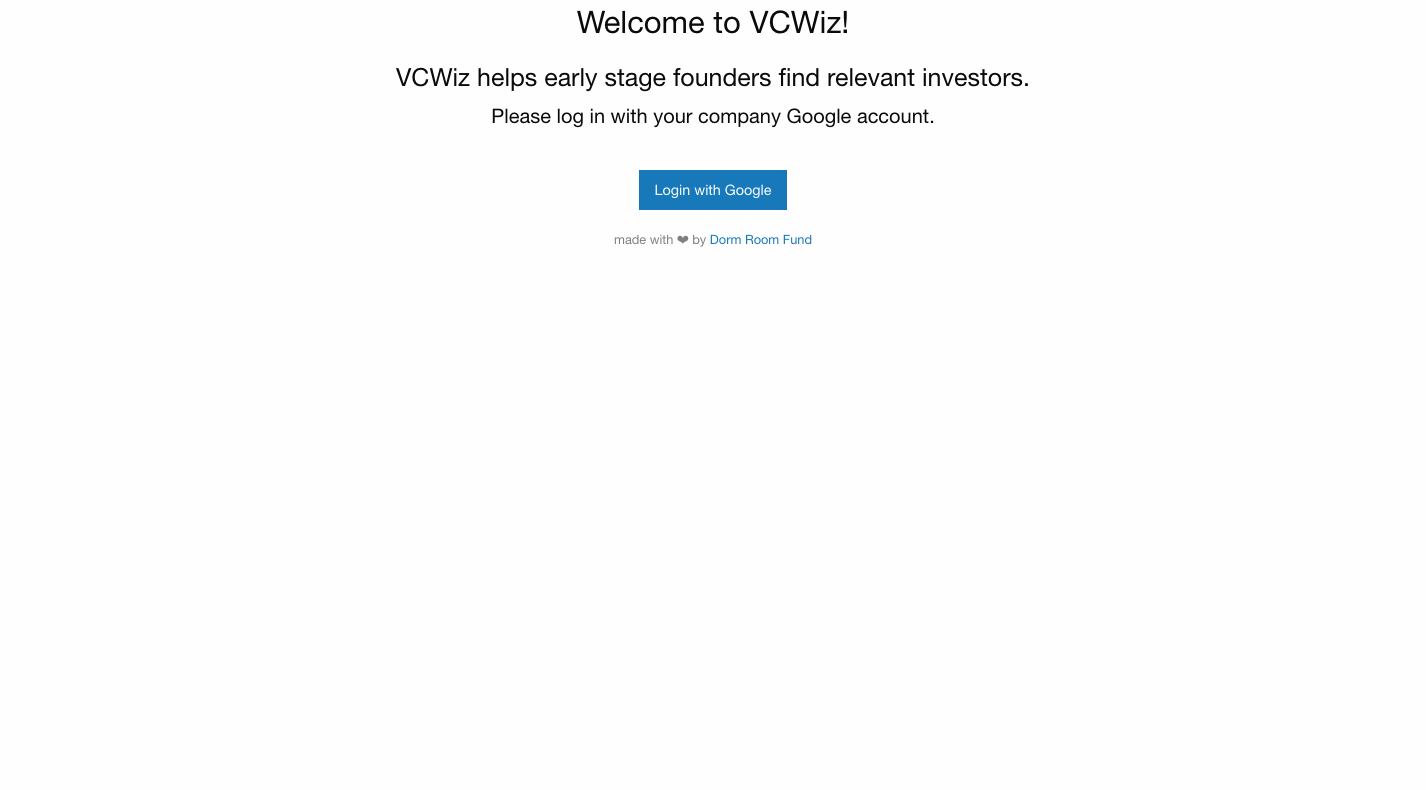
\includegraphics[width=0.9\textwidth]{vcwiz/v1/login.png}
    \caption*{Login Screen}
  \end{minipage}\hfill
  \begin{minipage}{0.33\textwidth}
    \centering
    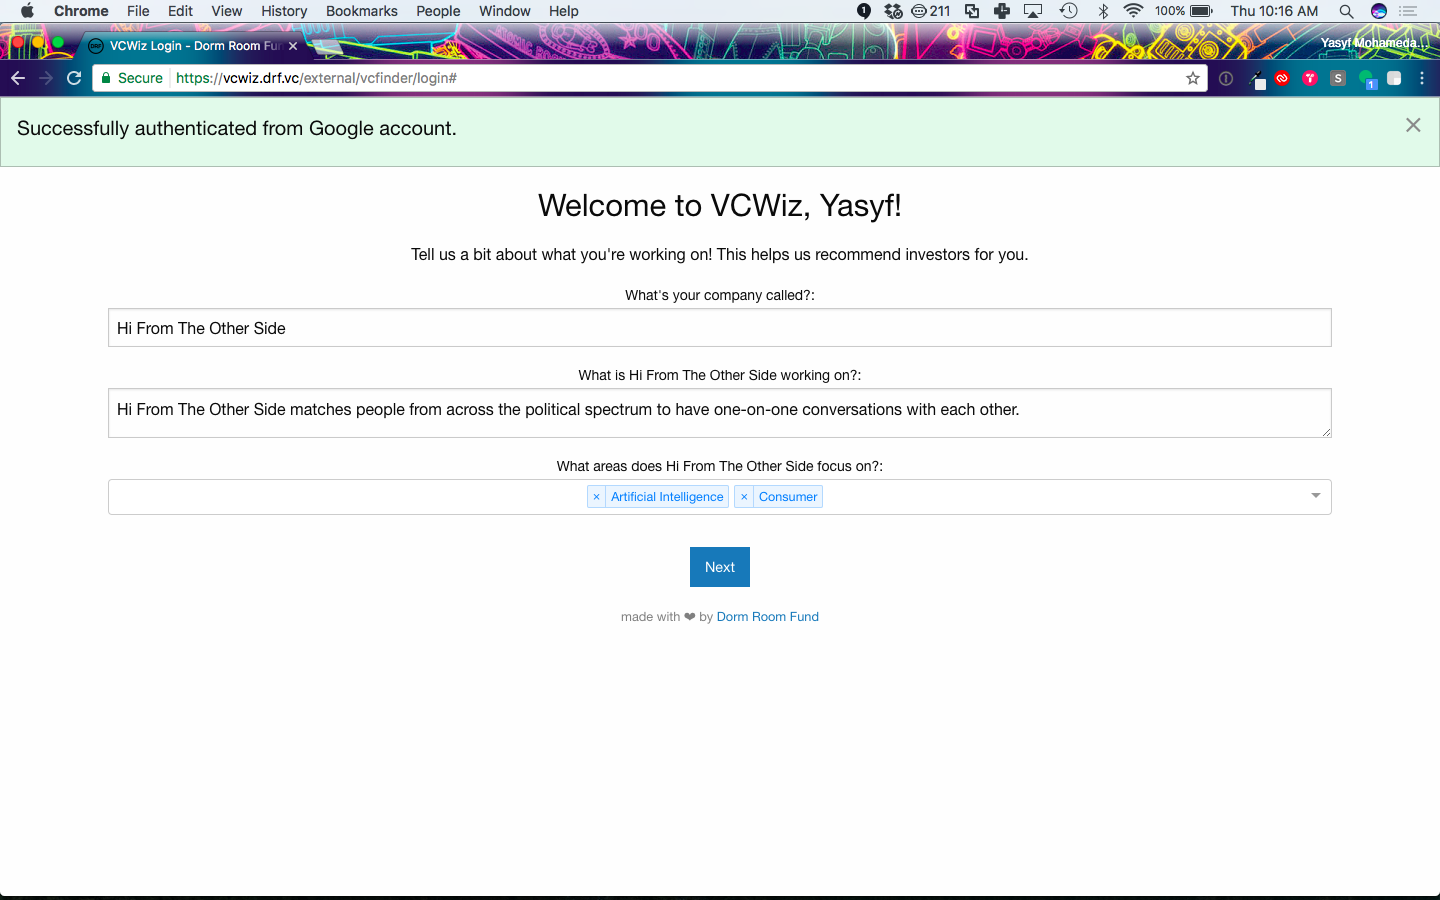
\includegraphics[width=0.9\textwidth]{vcwiz/v1/signup.png}
    \caption*{Signup Screen}
  \end{minipage}\hfill
  \begin{minipage}{0.33\textwidth}
    \centering
    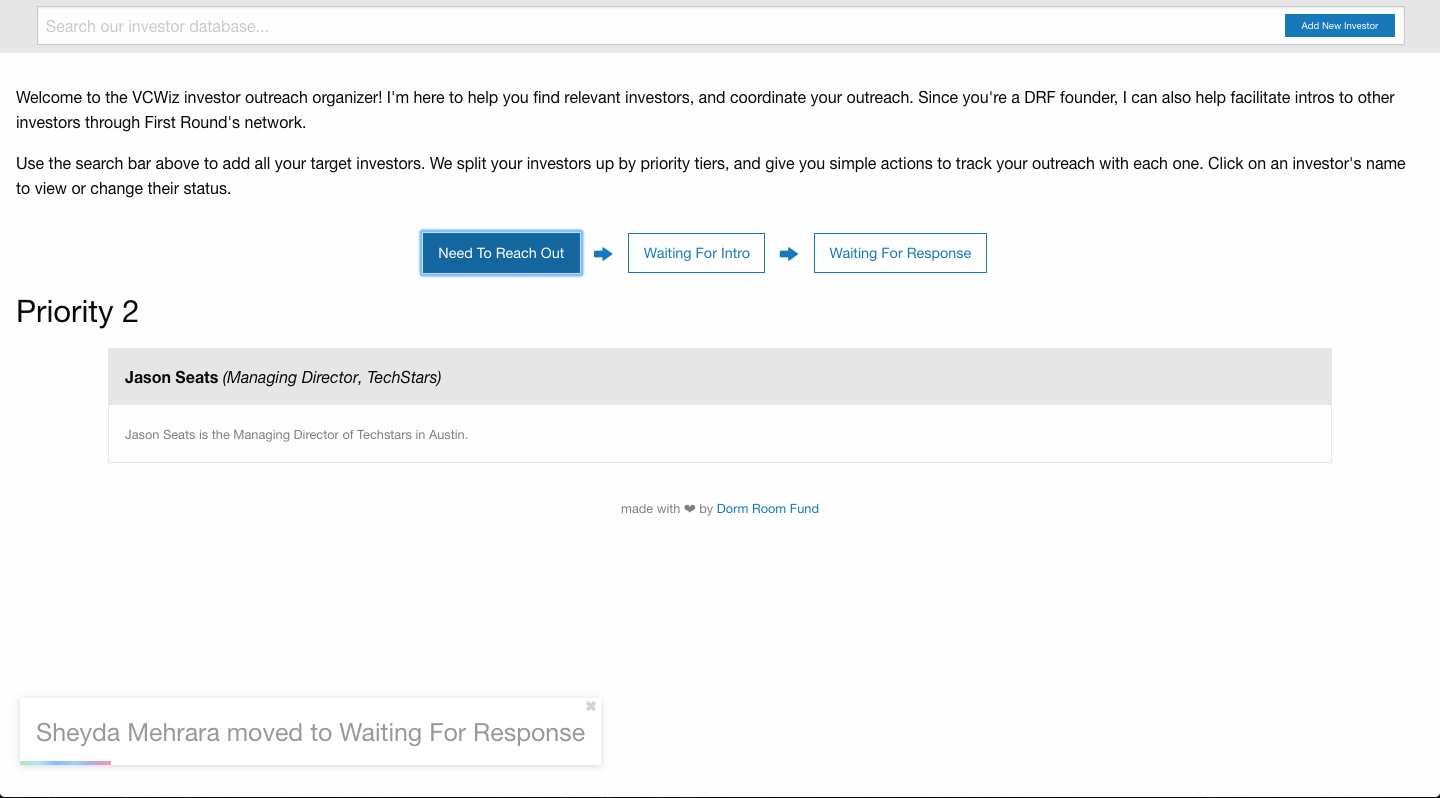
\includegraphics[width=0.9\textwidth]{vcwiz/v1/track.png}
    \caption*{Conversations}
  \end{minipage}
\end{figure}

\subsubsection{Feedback}

We learned a few crucial insights through the launch and test of this first iteration of the application.

With respect to discovery, we realized that founders do not find investors by looking at clusters of similar investors from a few seeds, as our model assumed. Instead, investors were found by examining the previous investors of similar companies to the one in question. While it meant that our kNN-based approach performed poorly for users, it reduced our discovery problem to a version of the very popular Netflix Prize~\cite{netflixpize} problem. Similar users (founders/companies) were positive about similar products (investors). We could now apply an entire body of recommendation-system research to the problem.

With respect to research, the biggest mistake we made was to include only a subset of the information we identified as useful for the founder. As a result, founders would end up leaving the platformt to do further research, which was disruptive to their workflow.

With respect to outreach, the first major learning was that it was very difficult to convince founders to trust us with their investor conversations, and that anything we could do to build credibility (for example, auto-filling form fields or leveraging the brands of the venture firms we were working with) vastly increased willingness to share data.

The next big learning was that our users were very familiar with a spreadsheet-based experience (either through Streak or with actual spreadsheets), and that trying to replace it was difficult and unnecessary. A very common piece of feedback was that a ``smart spreadsheet'' would be a far superior interface to the existing card-based workflow.

\subsection{V2}

\subsubsection{Design}

The second version of VCWiz was started in July of 2017. It featured a new recommendation engine, which first asked founders to identify competitors (or similar companies) which are more established. These companies were used to generate recommendations based on a simple algorithm, which takes the set of investors from the identified competitors, filters out the eligible ones, and sorts them based on their relevance, popularity, and whether or not they are featured. The popularity of investor $i$ is calculated based on the number of founders who have added $i$ to their outreach list.

\begin{lstlisting}[frame=single,mathescape=true,language=Ruby,basicstyle=\footnotesize,columns=fullflexible]
def recommendations(founder):
  investors $\gets$ founder.company.competitors.flat_map(c => c.investors)
  eligible $\gets$ investors.filter(i => i.industries $\cap$ founder.company.industries $\neq$ $\emptyset$)
  sorted $\gets$ eligible.sort_by(i => [i.featured, |i.industries $\cap$ founder.company.industries|, i.popularity])
  return sorted
\end{lstlisting}

Another addition to the second version was an augmented spreadsheet interface, which looks and feels like a spreadsheet, but auto-completes information about investors based on a VCWiz investor database. Once sufficient information had been entered on an investor into a row of the sheet to uniquely identify one record in the database, the remaining fields were filled. This gave the founders an experience they were comfortable with, with the power and ease of use they expected to justify switching tools.

In order to build up the VCWiz investor database, we started with a dataset imported from the Crunchbase Data Venture Program, then further augmented it with serveral additional sources. We will discuss our data pipeline in depth below.

The venture firms in our database are now tagged with the stage of company they invest in, based on the latest fundraising round that has occured. These categories are defined (and ordered) as such.

\begin{multicols}{2}
\begin{itemize}
  \item Accelerator
  \item Angel
  \item Pre-Seed
  \item Seed
  \item Series A
  \item Series B
  \item Venture
\end{itemize}
\end{multicols}

N.B. These categories are not necessarily mutually exclusive. For example, an accelerator may indeed give a startup their pre-seed round. The category for ``Venture'' captures all growth-stage companies (Series C and later).

Finally, we refined the stages a tracked investor could fall into, based on feedback from founders who were currently fundraising. The list below indicates the ordering over stages that is used throughout the platform.

\begin{multicols}{2}
\begin{itemize}
  \item My Wishlist
  \item Asked for Intro
  \item In Talks
  \item Need to Respond
  \item Pitching
  \item Committed
  \item Passed
  \item Not Interested
\end{itemize}
\end{multicols}

\begin{figure}[ht]
  \centering
  \begin{minipage}{0.45\textwidth}
    \centering
    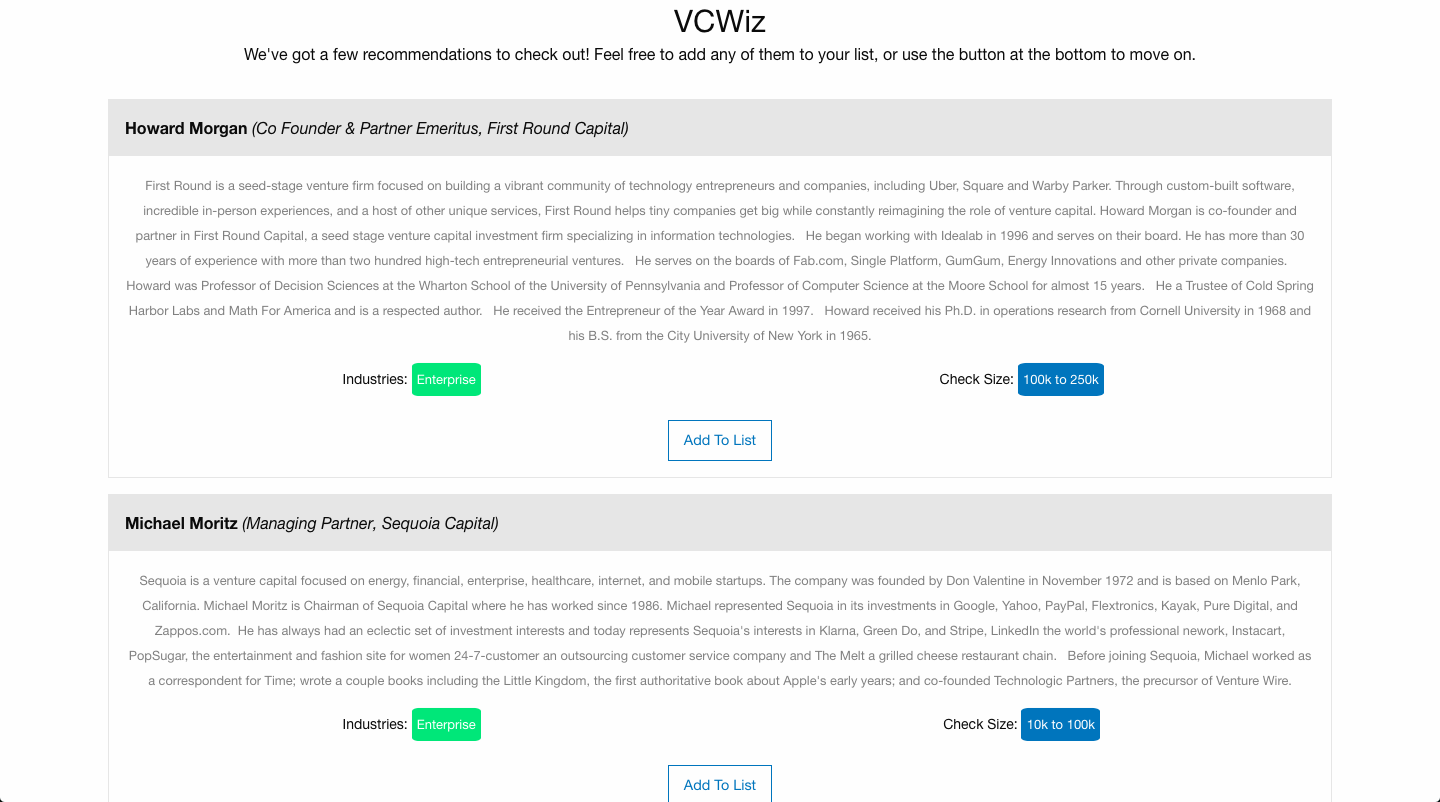
\includegraphics[width=0.9\textwidth]{vcwiz/v2/recommendations.png}
    \caption*{Investor Recommendations}
  \end{minipage}\hfill
  \begin{minipage}{0.45\textwidth}
    \centering
    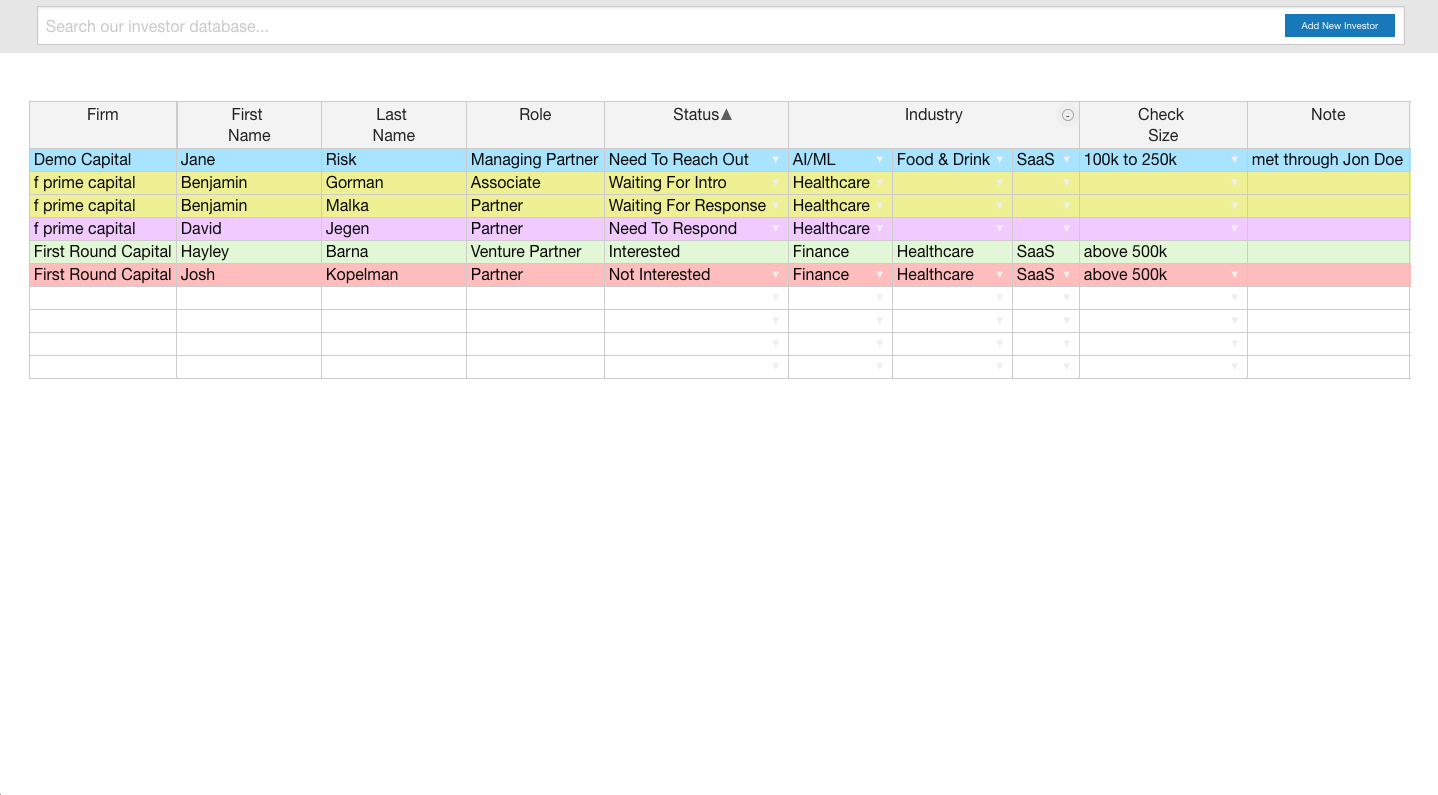
\includegraphics[width=0.9\textwidth]{vcwiz/v2/track.png}
    \caption*{Conversation Tracker}
  \end{minipage}
\end{figure}

\subsubsection{Feedback}

Following the completion of the second iteration of VCWiz, we did another series of user tests, asking founders to focus specifically on the improvements over the first version.

On discovery, the recommendations were not granular enough, and it was unclear why a certain investor was being recommended. Founders expressed the desire to filter and sift through investors with certain queries (such as some subset of the characteristics being used for recommendations), instead of being blindly handed what appear to be random investors. While there was still a desire for recommendations, it seemed that the place for this was after some amount of filtering, rather than in place of the filtering.

On research, it was felt that the platform still did not provide sufficient information to make it worth using over another tool. Nor did it display the little information it did show in an easy-to-digest way. A common suggestion was to incorporate content from social media and blogging platforms, as investors often use these platforms to demonstrate their interests.

On outreach, the major feedback was that the platform was too rigid. Having pre-defined stages and fields made it difficult to customize the tool for each founder's slightly different workflow, and made them feel like they were fighting the platform, instead of being empowered by it. A common feature request was some way to leverage mutual connections in the outreach.

We used Reichheld's Net Promoter Score (NPS) \cite{reichheld2003one} to track the growth potential of the product with respect to founders. At this stage, the product had an NPS of -50, which is very weak. Only 25\% of founders said they would recommend the product to a friend.

\subsection{V3}

The third iteration of VCWiz was started September of 2017, and aimed to incorporate all the previous feedback. The goal was for the end result to be a production-ready product that launches publicly. The interface and interactions were redesigned from the ground up, this time with the help of a professional designer. The functionality is still split across the three categories of discovery, research, and outreach, though each is now as feature-complete as the competing products which solve a narrower need. We embraced the feedback from fiunders that the product needed to be comprehensive and holisic, and have improved upon any of the popular features on other platforms.

We will first give an overview of the features of the third and final iteration of the platform, followed by an in-depth analysis of each component.

\subsubsection{Discovery}

VCWiz's initial screen contains an interface to filter and search for investors, by all the characteristics discussed previously, as well as by name and more novel metrics, such as topics often discussed. There are also options to constrain and modify the filters, such as changing a filter from a logical OR to a logical AND. In addition to the filtering and searching, there are curated lists of investors that meet specific criteria, ordered by popularity, and selectively shown to founders based on characteristics of their startup.

\subsubsection{Research}

Clicking through from any of the results in the filter view bring up a research screen which displays comprensive information on both a firm, as well as every partner at that firm. Every piece of information mentioned in interviews by founders as being useful is included in this view, including but not limited to biographies, social media links, recent investments, press mentions, blog posts and tweets, favorite topics to talk about, industries often invested in, and common co-investors.

\subsubsection{Outreach}

The outreach functionality of VCWiz is embedded in every screen, as well as having a decdicated dashboard.

Every tool for research and discovery has buttons to add investors and firms to the VCWiz Tracker, a CRM which is synced throughout the platform. Founders see a contextual dropdown showing the status of an investor in their pipeline any time they are researching that investor or their peers. The conversations screen is a dashboard which shows a table-like view, contiaining the information that was previously put in spreadsheets. We used a table to strike the balance between giving founders an interface they were familiar with, and displaying the information in a sufficiently detailed way. The data in this table is populated and updated through an integration with the founder's email provider.

In addition to merely tracking conversations, this version of VCWiz also overlays each screen containing details about an investor with a subset of the founder's email graph, showing them the shortest path(s) to the given investor in their network. This allows the founder to understand how likely they are to be able to reach an investor without a click.

The implementation and launch of this tool is detailed in the following chapter.

Shortly after the public launch of this third version of VCWiz on January 25th, 2018, we surveyed active founders on the platform to again calculate the NPS. This time, we received 117 responses, with an NPS of 0, a significant jump from the last version. 63\% of users agreed that they would recommend VCWiz to a friend, up dramatically from 25\% previously.

\begin{figure}[ht]
  \centering
  \begin{minipage}{0.33\textwidth}
    \centering
    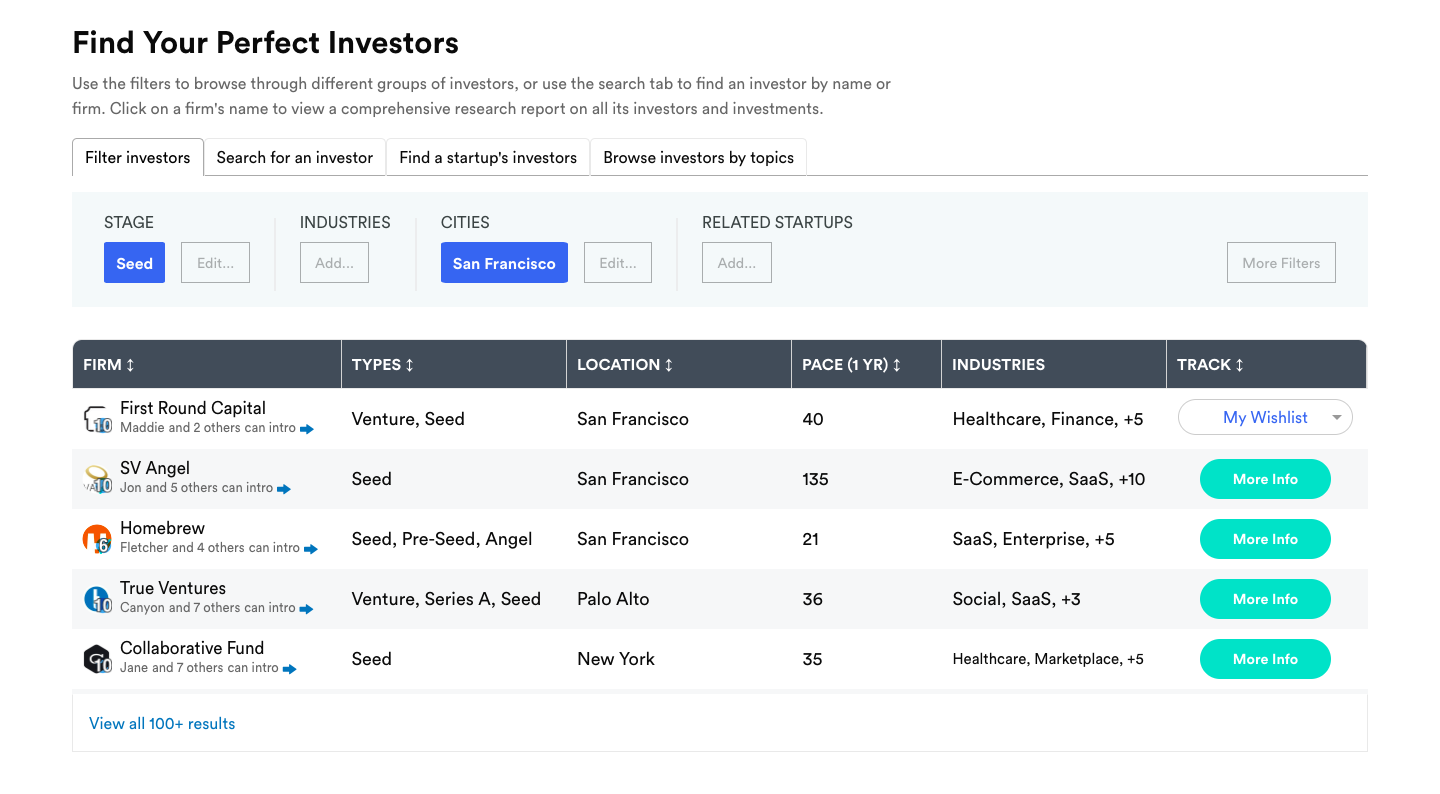
\includegraphics[width=0.9\textwidth]{vcwiz/v3/filter.png}
    \caption*{Filter \& Search}
  \end{minipage}\hfill
  \begin{minipage}{0.33\textwidth}
    \centering
    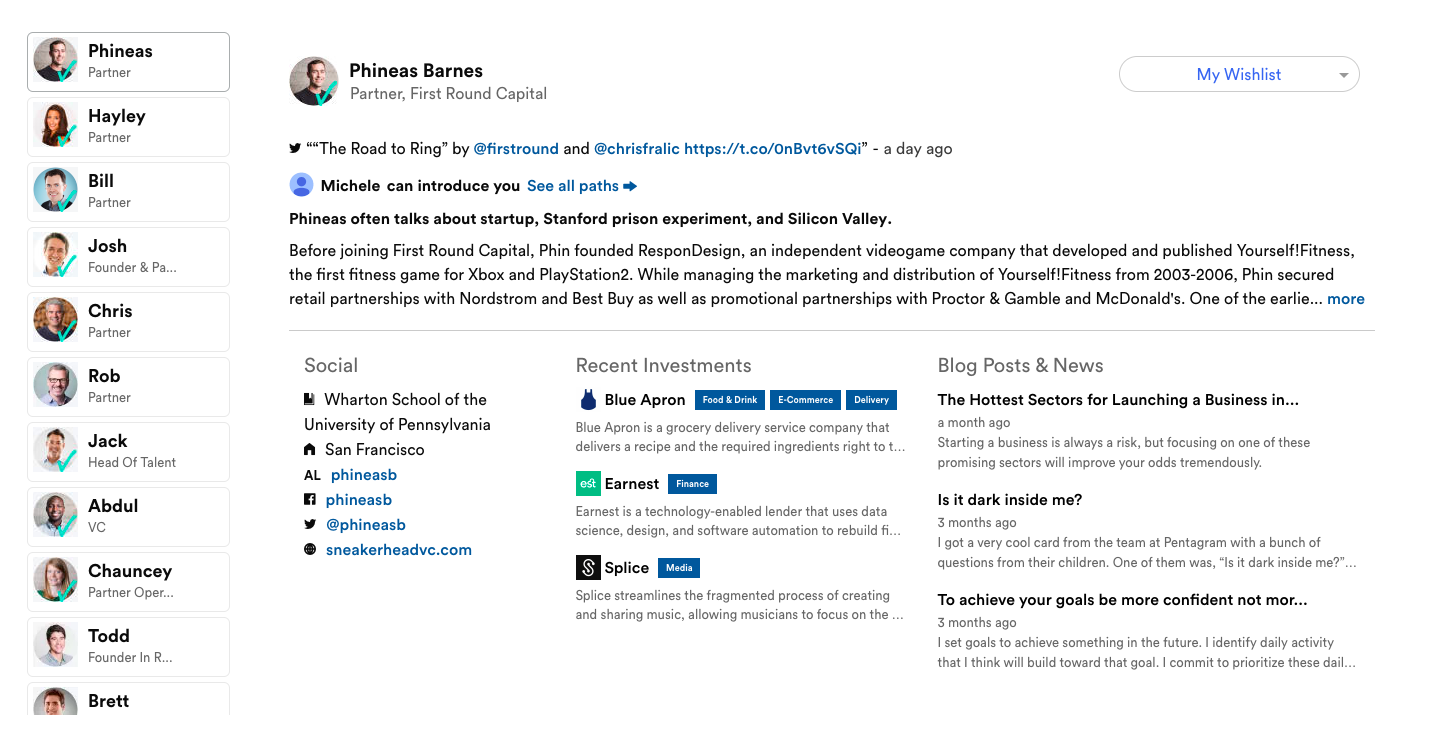
\includegraphics[width=0.9\textwidth]{vcwiz/v3/investor.png}
    \caption*{Investor Research}
  \end{minipage}\hfill
  \begin{minipage}{0.33\textwidth}
    \centering
    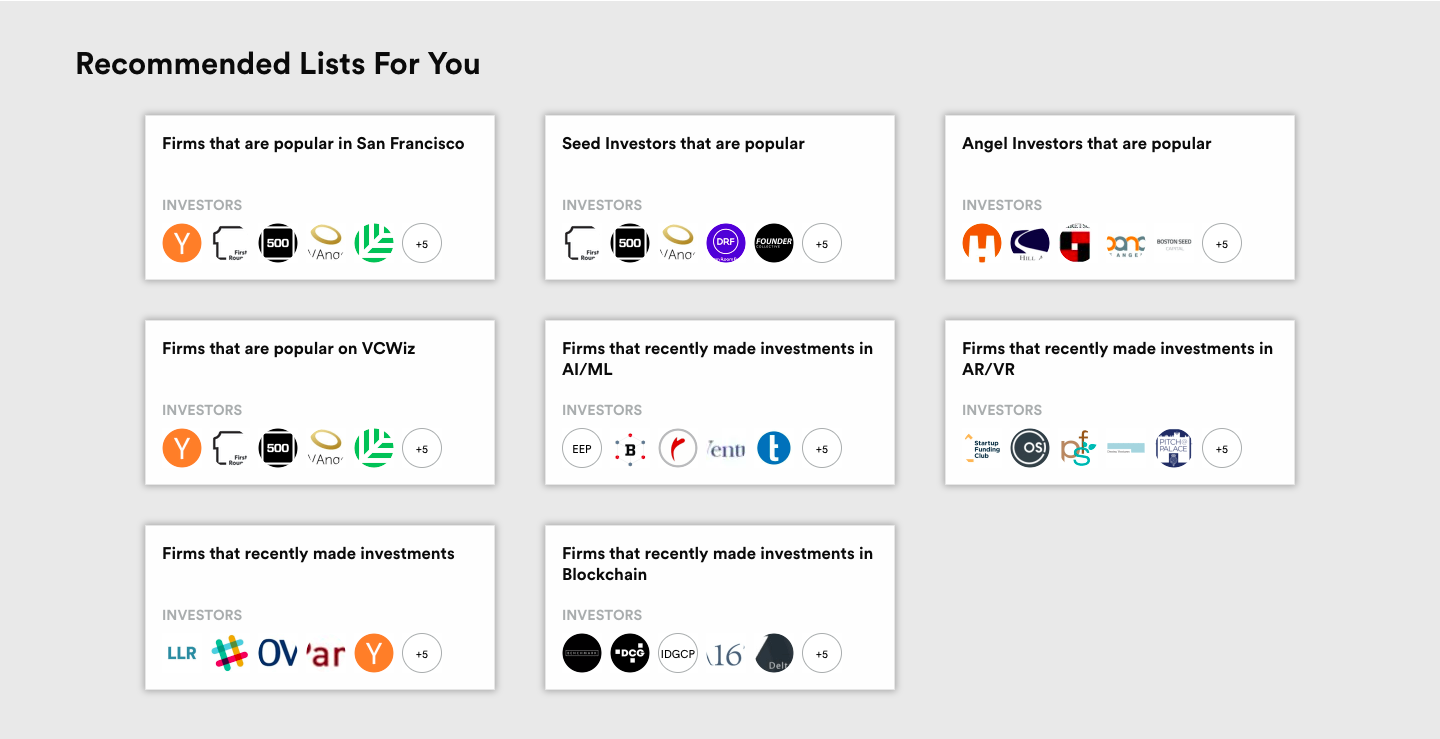
\includegraphics[width=0.9\textwidth]{vcwiz/v3/lists.png}
    \caption*{Curated Firm Lists}
  \end{minipage}
\end{figure}

\chapter{Final Tool and Launch}

This chapter will detail the final iteration of the VCWiz platform, and our efforts to launch it to the public.

\section{Final VCWiz Interface}

The final platform incorporated all the feedback from previous iterations, and was built over a span of four months. Below, we detail the technical details of the platform's interface, exploring each aspect in the order a new user would.

\subsection{Onboarding}

\begin{figure}[ht]
  \centering
  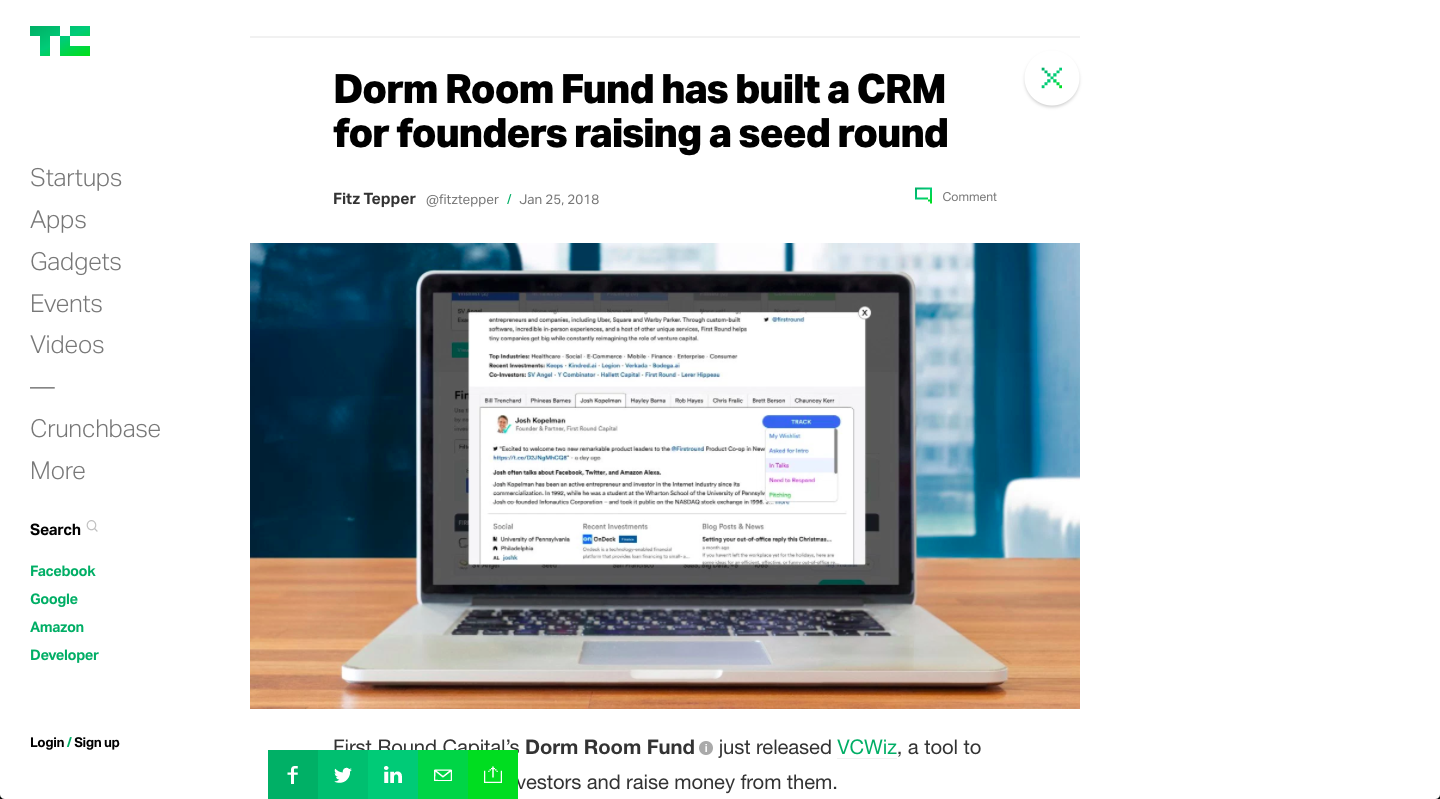
\includegraphics[width=\textwidth]{vcwiz/onboarding/techcrunch.png}
  \caption*{Launch on TechCrunch}
\end{figure}

Founders find the VCWiz platform through one of our launch partners (such as TechCrunch\footnote{\url{https://techcrunch.com/2018/01/25/dorm-room-fund-has-built-a-crm-for-founders-raising-a-seed-round/}}), or from search engines such as Google. We spent the months leading up to the launch generating research pages for every investor, firm, and company in our database (Figure \ref{screenshots:v3:onboarding}). These pages include comprehensive details on the entity in question, as described above, as well as an embedded view of all the VCs associated with that entity, and, if the user is signed in, all the personalization included in the platform.

After funneling users from their landing page to the main screen of the application, founders are able to filter, search, and explore lists of investors without creating an account. The site is fully functional from a discovery and research perspective, and about 80\% of users are content to peruse the content without creating an account. If the founder decides to create an account, we walk them through a series of questions to gather more information about their startup.

The signup flow begins by asking for the domain of the company. Using this as a unique identifier, we are able to query both our internal database, as well as external services (such as the Clearbit Logo API \footnote{https://clearbit.com/logo}) to gather as much information as possible on the founder's startup. The client browser makes a request to an API backend on the VCWiz server which initiates these requests in parallel, and returns a joined \texttt{Company} model within a given timeout threshold. This information is used pre-fill many of the following fields, including the name, description, industries, and competitors of the company. The founder is given a chance to verify this information, as well as provide mandatory information on their ideal investor profile. Finally, the founder is requested to log in with their Google account, in order to provide an authenticated email and social profile. We chose to use an OAuth2 \cite{hardt2012oauth}-based login flow with an existing service provider to simplify the login experience, and to avoid having to store user credentials. Google was the platform of choice on account of it providing verified email address information to users, as well as to unify the authentication experience in the case that the founder also decides to provide API access to their email inbox (for the purpose of synchronizing their conversations with investors).

Providing access to their email inbox is strictly an opt-in feature, and how the data will be used is explicitly described. As a result of our surveys to founders in previous iterations of the product, we found that it was necessary to have a plain-English description of our data use policy. We guarantee to founders that no human will ever read the individual messages of their inbox, that only aggregate data will be used for purposes other than their personal dashboard, and that we will only use metadata from their emails (headers, sentiment, etc.).  We allow ourselves to use features based on the body of the email, such as sentiment, provided they cannot be used to reconstruct a representation of the body.

After signing up, the founder is presented with a brief set of video clips that introduce the functionality to them (Figure \ref{screenshots:onboarding:intro}), including how to filter, search, and track investors. Following this, the site functions as it did before the founder signed up, with a few minor changes. Every screen with an investor has an integrated conversation tracker which shows the status of that investor, if any, in the founder's fundraise, as well as the email-based shortest intro path to that investor. The results of the filters are also personalized to the founder, based on the overlap in industries and location between each firm and the founder's startup. Signing up also unlocks the conversation tracker, with a preview of conversations on the main page (Figure \ref{screenshots:onboarding:summary}), and a dedicated screen for updating and viewing the status of each individual conversation (Figure \ref{screenshots:onboarding:conversations}).

\subsection{Ingesting User Data}
\label{vcwiz:ingesting}

One of the major insights from previous iterations of VCWiz was that founders have a variety of different ways they create and interact with data about their fundraising process, and they aren't often willing to change those. Thus, the tool we built had to meet founders wherever they currently were, in order to get their conversation tracker on our platform caught up. We built three independent tools for letting the system know about ongoing conversation, in addition to the integrations in the research and discovery sections.

The first (and easiest) way founders can import their conversations to the platform is to grant access to their Gmail inbox, either during the signup flow or when later prompted. This allows a regularly-scheduled job on our server to poll an API offered by Google \footnote{https://developers.google.com/gmail/api/}, and import new messages according to the pseudocode in Listing \ref{code:sync}. A \texttt{history\_id} parameter is cached in the \texttt{Founder} model to indicate the most recent thread fetched from Google, to avoid fetching duplicates in the future.

\begin{lstlisting}[float,frame=single,mathescape=true,language=Ruby,basicstyle=\footnotesize,columns=fullflexible,caption={Sync Inbox},label={code:sync}]
def sync_inbox(founder):
  for thread in fetch_threads(founder.address, founder.history_id):
    messages $\gets$ thread.fetch_messages()
    for message in messages:
      if message.from == founder.address:
        parse_outgoing(founder, message)
      else:
        parse_incoming(founder, message)
    founder.history_id $\gets$ thread.id
\end{lstlisting}

Parsing messages follows the algorithm in Listing \ref{code:parse}, which also augments the founder's email-based graph with every email processed.

\begin{lstlisting}[float,frame=single,mathescape=true,language=Ruby,basicstyle=\footnotesize,columns=fullflexible,caption={Parse Message},label={code:parse}]
def parse_message(message):
  if check_if_bulk(message):
    return
  founder.graph.connect(message.address)
  target_investor $\gets$ find_or_create_target_investor(founder, message)
  if !target_investor:
    return
  if !target_investor.email:
    target_investor.email $\gets$ message.address
  target_investor.stage $\gets$ guess_stage(message)
  create_new_email(founder, target_investor, message)
\end{lstlisting}

As can be seen from the algorithm, when importing a user's emails and creating their email graph, we first started with the naive approach of scanning every email, creating a node (if one did not already exist) per address, and creating outgoing edges every time one node sent an email to another. While this works when only importing emails once, the APIs at our disposal were imperfect. The \texttt{history\_id} tracked from Google's API often expire, and imports must be repeated. Thus, we had to start tracking a unique message identifier in our own database to ensure emails are imported at most once.

There were also several heuristics we used to skip messages that could be classified as bulk mail, as this added a lot of noise to the dataset. If the message meets any of the following criteria, it is logged and skipped. The full algorithm can be found online \footnote{https://git.io/vxunk}. In these criteria, the recipients are defined as the union of the TO, CC, and BCC fields, and body is defined as the concatenation of the text and HTML sections of the message.

\begin{itemize}
  \item There are more than 5 recipients
  \item The body contains a phrase often used in bulk mailings, such as ``unsubscribe'', ``terms of use'', or ``view in your browser''
  \item The headers contain one of several common listserv headers, such as List-Unsubscribe and many vendor-specific ones
  \item The return path of the message includes a popular bulk email vendor
  \item The local component of the from address is that of a commonly-automated inbox, such as ``noreply'' or ``info''
  \item The name of the sender includes common aliases, such as ``support'' or ``payroll''
  \item The domain of the sender or any recipient is one that is common in transactional emails
\end{itemize}

The second way founders can inform the system about ongoing conversations is to CC (or BCC) a special email address, which routes to a server which accepts the message and forwards the relevant metadata to an API endpoint on VCWiz. This metadata is parsed and the email is reconstructed, before being run through the same algorithms as above. This alternate, manual way of updating VCWiz via emails was added for the more privacy-conscious founders on the platform, who wished to have the convenience of updates based on emails without handing over access to their entire inbox.

The third and final ways founders can update the system in bulk is by uploading a existing spreadsheet of conversations. Our surveys revealed that the most commonly-used tool for tracking conversations with an investor was a spreadsheet (or spreadsheet-like tool), so providing an easy way to migrate those onto the platform was essential. Founders can export a CSV file from any spreadsheet-based tool and import it on the conversation tracker page of VCWiz. The server parses the rows out of the CSV, and uses both the format of the content of a column as well as it's header (based on the Levenshtein distance \cite{1966SPhD...10..707L} of a given header from a list of common choices) to guess which columns correspond to which internal database columns of a \texttt{TargetInvestor}. This mapping is presented to the founder for verification (Figure \ref{screenshots:import:columns}), and then is used to import the rows as a background job.

\subsection{Filtering \& Searching}

\subsubsection{Filtering}

The main filtering interface of VCWiz allows founders to display investors that match a set of criteria. We will detail each of those criteria before describing the algorithm used to filter. The logic behind the selection of criteria is to cover the majority of the ways founders describe their ideal investor: the stage the investor operates at, the industries that they invest in, the location they invest in, and their relationship to similar/competing companies (similar companies are generally a good sign, whereas directly competing companies might be prohibitive).

The first criteria is based on the stage of the company, as defined by it's latest funding round. It is a filter on the funding round a venture fund invests in, either as reported by the fund, or based on their past investments. Note that a fund can have multiple stages affiliated with it, as can a funding round of a company (often in the cases of ambiguity); when aggregating past investments, any stage which shows up at least half of the time is attributed to the fund. This criteria is always a logical \texttt{OR} when multiple are selected.

The next criteria is the set of industries that a fund commonly invests in. Once again, these are preferably self-reported, and there can be multiple associated with a fund (as well as an investor or a company). They are aggregated in the same was as the stage. The set of industries are fixed: there is no free-form option when filtering. The set of industries to display as options \footnote{https://git.io/vpTbj} was selected using the algorithm in Listing \ref{code:industries}, on all the companies in the Crunchbase data set. The goal is to select the set of industries that cover the entire set, with minimal overlap.

\begin{lstlisting}[float,frame=single,mathescape=true,language=Ruby,basicstyle=\footnotesize,columns=fullflexible,caption={Display Industries},label={code:industries}]
def covering_industries(companies):
  all_industries $\gets$ companies.flat_map(c $\to$ c.industries)
  industry_options $\gets$ all_industries.unique()
  sorted_options $\gets$ industry.sort_by(i $\to$ all_industries.count(i))

  selected $\gets$ set()
  while companies.filter(c $\to$ c.industries $\cap$ selected $\neq \emptyset$).count() > 0:
    selected $\gets$ selected $\cup$ {sorted_options.pop()}

  return selected
\end{lstlisting}

By default, when a founder selects multiple industries, the filter is a logical \texttt{OR} of these industries. However, there is an option which can be toggled to make this filter an \texttt{AND}, such that returned companies have to invest in \textit{all} the specified industries.

The next criteria is based on a set of cities. By default, this filter returns firms which are based in the cities specified (firms have a single headquarters, and an array of locations, which are both matched against). There is an option, however, to change this filter to instead return firms that have invested in \textit{startups} based in the specified city (each startup is affiliated with a single city).

Another criteria to be matched against is a set of relevant startups. The founder can select this set from the database of companies VCWiz tracks internally. By default, this set restricts the returned firms to those who have invested in at least one of the specified companies. An option can be toggled which changes this filter to restrict to the set of firms that have invested in \textit{similar} companies, based on the industries of each company in the set.

The final criteria to match investors against is a set of topics. In this case, a topic is anything found in the VCWiz entity database, built up by extracting entities from the various data sources discussed elsewhere. At the time of writing, this database contains $98,000$ records. The filter based on these entities is a logical \texttt{OR}, and will return investors who often mention or discuss any of the given topics. In this case, we include a topic for an investor if that topic is mentioned at least 5\% of the time in content created by or mentioning the investor.

Finally, here is a lone option to restrict the returned set of investors to those that operate solely in the US. This was a popular criteria for many founders on our platform.

\subsubsection{Searching}

In addition to filtering against any combination of the above criteria, founders can also filter investors based on the name of the firm or individual investor. This is implemented as a simple fuzzy string match on the \texttt{name} field of \texttt{Firm}, and the \texttt{first\_name} and \texttt{last\_name} fields of \texttt{Investor}.

\subsubsection{Sort}

Once VCWiz has generated the set of investors that match each filter and search query, it must decide the order in which to display the results. There is a custom ranking function which sorts the results, using each metric as the tie-breaker for the last.

\begin{enumerate}
  \item If the topic filter is present: the number of investors in the firm which match the set of topics
  \item The number of ``featured'' investors in the firm
  \item If the industry filter is present: the number of intersecting industries between the firm and the query
  \item If the city filter is present: the number of intersecting cities between the firm and the query
  \item The number of founders on the platform who have initiated a conversation with the firm
  \item The number of ``verified'' investors in the firm
\end{enumerate}

N.B. Any metric which does not have it's requirement met is simply ignored. ``Featured'' investors are those on the platform who have been hand-picked as high-quality investors. ``Verified'' investors are those who have completed their investor profile on VCWiz self-reported their characteristics.

This sort achieves personalization by using the industries of the founder's startup and current location of the founder for the purpose of sorting, when the respective filters for those characteristics are not specified. Thus, if a founder specifies all the possible filters, they will get the same results that any other founder who does the same will. However, if the relevant filters are unspecified, information from the founder's profile will be used for ranking and displaying the results, giving a different ranking than some other founder.

The interface displayed to the founder also allows for manual sorting of the results based on the natural ordering of a given column. If this overriding sort is provided, none of the above is used.

\subsubsection{Implementation}

The algorithm for displaying the results of this process \footnote{https://git.io/vpkvd} is demonstrated in Listing \ref{code:filter}.

We start with every firm in the database, and filter out any that do not match the search terms provided by the founder. Often, the search term is given as a single query string. In this case, we treat this string as both the query for the firm name, as well as the investor name (the first word of the string is considered the query for the first name, and the remainder for the last name). Any individual investors who match have their firms added to the results.

Following the search query, we apply every present filter to the remaining set of firms, narrowing down the result set each time.

\begin{lstlisting}[float,frame=single,mathescape=true,language=Ruby,basicstyle=\footnotesize,columns=fullflexible,caption={Filter and Search},label={code:filter}]
def filter_and_search(all_firms, founder, filters, search):
  firms $\gets$ all_firms
  investors $\gets$ firms.flat_map(f $\to$ f.investors)

  if search:
    first_name, last_name = extract_name_components(search)
    investor_by_name $\gets$ investors.filter(i $\to$
      i.first_name.contains(first_name) || i.last_name.contains(last_name)
    )
    firms_by_investor_name $\gets$ investor_by_name.map(i $\to$ i.firm)
    firms_by_name $\gets$ firms.filter(f $\to$ f.name.contains(search))
    firms $\gets$ firms_by_name $\cup$ firms_by_investor_name

  for filter in filters:
    firms $\gets$ apply_filter(firms, filter)

  sorted $\gets$ apply_ordering(firms, founder, filters)
  return sorted
\end{lstlisting}

\subsubsection{Display}

The results from the filtering and searching process are displayed in an infinitely-scrollable table to the founder (Figure \ref{screenshots:filtering:results}), with the following columns.

\begin{enumerate}
  \item The name and photo of the firm
  \item The company stages the firm invests at
  \item The headquarters of the firm
  \item The number of investments the firm has made in the last calendar year (``pace'')
  \item The top three industries that the firm invests in
  \item A drop-down to add or update the firm in the conversation tracker
\end{enumerate}

N.B. What founders really desire to see in the ``stage'' column is the average cheque size of the firm. However, this number is difficult if not impossible to calculate given the limited public data on investor contributions to a given fundraising round. Thus, the company stage is used as a proxy.

The ``pace'' column is present to give the founder a sense of how active a given firm is. This was added by popular request after many founders found it difficult to determine whether or not a firm was still actively investing their current fund.

Each column (other than ``industries'') also provides a button for overriding the ranking function. This allows the founder to view the result set, sorted by only the data in the particular column. The ``firm'' and ``location'' columns are sorted lexicographically, the ``pace'' column numerically, and the ``stage'' and ``track'' columns by their inherently-defined orderings.

In the case where a search query is specified, or the topic filter is used, it is valuable to not only surface not only the resulting firms, but the best-matching investor at each firm (e.g. if the search query matches the first name of a partner). In these cases, there is an additional, non-sortable column titled ``Partner'', which displays the name and photo of that best match (Figure \ref{screenshots:filtering:partner}).

\subsubsection{Initialization}

When a founder first completes the signup flow for VCWiz, they are presented with a page containing functional real-time filtering, according to the above. To ensure a positive first experience viewing the results of filters, we make a few assumptions, and initialize the founder's filters to what we believe are sane defaults. We set the funding round filter to ``Seed'', to reflect the target user of the platform. The industry and relevant startups filters are pre-filled with the industry and competitors of the founder's startup, respectively. Finally, the location filter is set to the nearest ``hub city'', relative to the founder's current location (based on their IP address). A ``hub city'' is defined as a city that has at least 50 venture firm offices (as reported by VCWiz) within it.

\subsection{Introduction Requests}
\label{chap4:introrequests}

One experimental part of the final VCWiz platform was the ability for founders to request introductions to out-of-network investors on the platform.

The motivation behind this was to standardize the format and medium of ``cold'' intro requests in the venture community. As discussed earlier, there is both qualitative and quantitative data supporting the use of mutual connections to make introductions when reaching out to investors. This is corroborated by the results of our experiments on the VCWiz graph, which indicate that how central a founder is in the global social graph of startups and venture capital is highly correlated with how easily a founder will raise money. However, sometimes this is simply not an option. In this case, founders resort to ad-hoc, unsolicited emails to investors, leveraging myriad folklore tactics to increase the chances of a response. This is a frustrating experience for both parties: investors are deluged with a stream of unwanted pitches, mixed haphazardly into their daily business, while founders are disappointed that their carefully-crafted custom email gets lumped in with the bulk email another founder sent to 1000 investors.

We attempted to solve this problem by providing a tool for founders to send a templated introduction request, which looks identical each time (save for a customizable blurb), to an investor (Figure \ref{screenshots:intro:request}). The investor's email address is never initially revealed to the founder. Instead, a request email is sent by the VCWiz platform to the investor, containing an automatically-generated dossier on the founder and their startup (from the information provided at signup). The investor can respond to this automated email with a simple ``yes'' or ``no'', and only in the case of an affirmative response is a second email sent from the platform, connecting the founder and the investor.

While many investors agreed that using an automated third-party such as VCWiz was preferable to founders directly sending countless emails and followups, there was significant doubt that such a platform would be adopted to such a degree that it could be considered a success. As it turns out, these concerns were well-founded. When we launched the feature, we were tracking a funnel of four success metrics:

\begin{enumerate}
  \item The number of introductions requested
  \item The number of requests which receive a response
  \item The number of successful connections
  \item The number of investments made as a result of an introduction
\end{enumerate}

N.B. a ``successful connection'' is defined as any introduction which results in at least one additional email from each party.

A few months after launching the feature, we saw the following usage. Out of 301 introductions requested, only 19 garnered a response from the investor, of which five were affirmative. One of these resulted in a successful connection, and none resulted in an investment.

Our hypothesis was that this experiment failed for two reasons. The first was that the founders who resorted to using this tool were inexperienced at fundraising or were not very well-connected, which presents an adverse selection problem: as we will demonstrate later, founders who are not well-connected will struggle to raise relative to those who are. The second reason was that investors have such a low response rate to cold emails of any kind that any improvement was negligible.

We tested this hypothesis by surveying every founder on the platform, and every one of the 247 investors who had received an introduction request.

We asked the founders why they had or had not used the introduction request feature. 118 founders responded, with 10\% saying they had tried the feature, 23\% saying they would never get a cold introduction to an investor of any form, and 16\% not understanding the value of the feature. The long tail of remaining responses ranged from not currently needing any intros, to hitting bugs when trying to use the feature. This data supports that many founders are skeptical of using the feature, or any cold introduction, because of how ineffective they are. The majority of these founders (65\%) have exchanged emails with investors before, indicating they are the more seasoned founders.

Only 13 investors responded to the investor survey, but the overwhelming response was that the founders who had reached out were simply not high quality, or a good fit for their fund. This supports our hypothesis about founders, and the very fact that there were so few responses corroborates our hypothesis about investor response rates to unsolicited emails. An interesting corollary to a few of the responses was the realization that our solution still inconvenienced investors more than they would like. The ideal solution would involve a centralized dashboard of requests which could be checked for interesting prospects by designated individuals at the firm, often not the investors themselves.

\subsection{Intro Paths}

Founders who have shared their email graph with VCWiz can see their ``Intro Path'' to any given investor on the platform (Figure \ref{screenshots:intro:path}). The goal of displaying these paths (and the length of that path as investor's distance from the founder) is to assist founders in planning who can make an introduction for them (so as to avoid the problem discussed above).

This path is calculated by running a standard single-pair shortest-path algorithm between the founder's node and the investor's node. If multiple paths are found, the paths are ranked by the strength of the connections they represent (based on the sum of the frequencies of emails between nodes on the path), and the top three are returned. The Cypher script run on our Neo4j database instance to accomplish this has been reproduced in Listing \ref{vcwiz:cypher:intro} (p. \pageref{vcwiz:cypher:intro}).

Intro Paths are also available between founders and venture funds. In this case, the same algorithm as above is run, for every investor within the fund. We take the union of the resulting shortest paths, and rank them in the same way.

\section{Final VCWiz Backend}

The architecture of the final VCWiz application comprises of a Ruby on Rails\footnote{http://rubyonrails.org/} application which serves both the frontend React\footnote{https://reactjs.org} application and an internal API. Data on firms, investors, companies, and founders is ingested from many sources on a regular basis, using Sidekiq\footnote{https://sidekiq.org/}, a job scheduler, to update specific shards of the database at a time.

% A summary of the jobs can be found in \ref{vcwiz:jobs}.

The main persistent store for data is a PostgreSQL\footnote{https://www.postgresql.org/} database running on Amazon Web Services (AWS). There are also instances of Redis\footnote{https://redis.io/} (for caching external API responses), Memcached\footnote{https://memcached.org/} (for caching internal intermediate data for rendering), and Neo4j\footnote{https://neo4j.com/} (for calculating Introduction Paths).

The application servers are deployed on Heroku\footnote{https://www.heroku.com/}, a platform-as-a-service which is also running on AWS.

Below, we detail the various aspects of the backend, and how data flows through the system.

\subsection{Data Models}

The main data models in VCWiz are the \texttt{Company}, \texttt{Founder}, \texttt{Investor}, \texttt{Firm}, and \texttt{Investment}. These, along with auxiliary models, are diagrammed in Figures \ref{vcwiz:model:hierarchy} and \ref{vcwiz:model:content}. N.B. In the diagram, \texttt{Firm} is referred to as \texttt{Competitor} for legacy reasons. Each of these models is backed by a similarly-named database table.

The decision was made to have many \texttt{Company}s per \texttt{Founder}, as founders on the platform very often have started a company before. This leads to the denormalized \texttt{PrimaryCompany} model, which simply keeps track of which \texttt{Company} is the one a founder is currently leading. One current issue with the platform that results from this is that any founder can claim to be affiliated with a startup already in the system, whether or not this is true.

Each founder can own many \texttt{TargetInvestor}s, which represent a conversation between a founder and an investor (or an investor on a founder's wishlist). \texttt{IntroRequest}s and \texttt{Email}s are then affiliated with a \texttt{TargetInvestor}.

Tweets, news articles, and blog posts mentioning either an individual investor or entire firm are each tracked by their own model. An \texttt{Entity} model that can be associated with any of these tracks mentions of extracted entities from the content, and is used for topic-based searching. In order to reduce noise in the selection of entities, we made the decision to only create an entity record if a given entity has an entry on Wikipedia \footnote{https://www.wikipedia.org}.

\subsection{Data Pipeline}
\label{ch4:data}

There are several sources of information used by the data pipeline in VCWiz, each of which is abstracted, normalized, and merged into the existing schema of the system.  Instead of attempting to mirror the structure of each API in the server code, a wrapper class (\texttt{ApiObject} \footnote{https://git.io/vpvib}) was created, which abstracts away common structure in the external API endpoints accessed. This allows simple property-based access of the JSON objects returned, with automatic detection of arrays and types which need to be converted (such as dates). The general method for building up profiles of objects in VCWiz is to start with a base source of truth (often Crunchbase), then augment these objects with a variety of information streams, some of which are documented below.

\subsubsection{Crunchbase}

Through the Crunchbase Data Venture Program, we received access to the entire database of investors, firms, and companies on Crunchbase. Each \texttt{Company}, \texttt{Founder}, \texttt{Investor}, and \texttt{Firm} on VCWiz stores a unique Crunchbase identifier (\texttt{crunchbase\_id} or \texttt{cb\_id}), which allows changes on Crunchbase to be reflected in VCWiz models (when appropriate). Whenever an object with associations that have Crunchbase identifiers is updated, background jobs are initiated which attempt to fetch updates for each association. Furthermore, approximately once a month, a complete dump of the Crunchbase database is downloaded and imported (skipping over existing records).

\subsubsection{AngelList}

Each \texttt{Company}, \texttt{Founder}, \texttt{Investor}, and \texttt{Firm} also has a field for storing an AngelList identifier. The AngelList API \footnote{https://api.angel.co} is used to augment information on these objects when Crunchbase is ambiguous or incomplete. Through manual inspection, we found that AngelList's dataset often contains more information for companies which are so early-stage that they have not yet raised money from institutional investors, whereas Crunchbase focuses on venture-backed startups.

\subsubsection{Bing News Search API}

The Bing News Search API \footnote{https://azure.microsoft.com/en-us/services/cognitive-services/bing-news-search-api/} is used to periodically check for previously-unseen news articles on a given investor. These news articles are imported and processed, which involves summarizing them, extracting entities from their bodies, and categorizing their sentiment. All of this information is saved to a \texttt{News} record, which is displayed to users on the research page for a \texttt{Investor}.

\subsubsection{Newsriver}

Newsriver \footnote{https://newsriver.io/} is a similar API to Bing News Search, and is also used to monitor for new press on an investor.

\subsubsection{Clearbit}

Clearbit \footnote{https://clearbit.com/} is a service which provides access to a dense graph of human profile information, with nodes that can be identified with an email address or social media profile. We use it to auto-fill parts of the profiles on VCWiz, both for founders and investors.

\subsubsection{Text Processing API}

We use the Text Processing API \footnote{http://text-processing.com/docs/} for entity recognition and sentiment analysis of many pieces of text, including news articles and emails.

\subsubsection{Google Cloud Natural Language}

We use the Google Cloud Natural Language API \footnote{https://cloud.google.com/natural-language/} for the same reasons as the Text Processing API.

\subsubsection{Hunter}

Hunter \footnote{https://hunter.io/} is a service which collects common email patterns on a per-domain basis to aid in guessing a person's email address given their name and domain. When a founder requests an introduction to an investor who has not yet signed up for the platform, we use Hunter to guess their email.

\subsubsection{Twitter}

We use the APIs provided by Twitter \footnote{https://developer.twitter.com/en/docs} combined with the social media usernames reported by Clearbit to log recent tweets of every individual investor on the VCWiz platform. These tweets are displayed on the research page for the investor. Entities are extracted from these tweets, and are used to build a profile of the topics affiliated with an investor.

\subsubsection{Medium}

Medium \footnote{https://medium.com/} is a popular platform for blogging. When an investor has a profile on Medium, it is scraped regularly to identify new blog posts to display on the research page. Like tweets, entities are also extracted from blog posts for analysis.

\subsubsection{Homepages}

The homepages of investors, firms, and founders are all scraped for entity extraction, similar to the blog posts and news articles above.

\subsection{Inferring Partners}
\label{ch4:partners}

One of the most useful pieces of information about a given venture fund is which partners at the fund have been the leaders of which deals. There is huge variance in the industry, business model, and founder background that each partner of a firm prefers, and selecting the right one can vastly improve the chances a founder finds the right fit in an investor. Unfortunately, it is not common practice to make public which investors are the point partners on each deal done by the firm. Thus, founders are often left in the dark.

One of the key insights we had while building VCWiz is that there are often sufficient signals online to infer which partner at a firm was responsible for a given investment. These signals include the partner mentioning a portfolio company in their biography, frequently tweeting about a company, or often commenting to the press on behalf of the firm on matters regarding a company. While aggregating these signals manually would be tedious and difficult, it is a very easy process to automate. Thus, our backend periodically queries for press and social media mentions of the portfolio companies of each firm, and scans those mentions for the names of the partners at the firm. If a partner appears more often than others, we assume they are the partner responsible for the investment.

While this method is not perfectly accurate, it has empirically been sufficient.

\subsection{Security}

The dataset and internal API endpoints exposed by VCWiz present a large opportunity for abuse. The resources required to build and maintain the database of investors, firms and companies are considerable, and every other site which presents a similar dataset goes to great lengths to discourage web scraping and other illegitimate access. Often, sites will employ the services of a company such as Distil Networks \footnote{https://www.distilnetworks.com/}, which uses a variety of Javascript-based methods to make it difficult or impossible to programmatically get the HTML of a webpage. Since VCWiz exposes a JSON API to the public internet, it was necessary to take precautions against anything other than the VCWiz frontend accessing internal resources. Furthermore, additional measures were put in place to make sure no one could access a founder's data, other than that founder themselves.

The security of the entire application is handled through a few efforts. All data is stored in a single database, with credentials stored as an environment variable on the web server. These credentials are rotated automatically on a regular basis. Any API keys or further credentials are also stored as environment variables, never recorded in code. User sessions are encrypted with a private key only held by the web server, and serialized into client cookies. These sessions contain the primary key of the currently logged-in \texttt{Founder}, if any, and is used to ensure that no one can access a founder's data without authorization.

When it comes to the API specifically, we want to prevent both unauthorized reads (of user or bulk data) and writes (that a user did not intend).

Writes across founders are defended against with the measures described above. A common attack vector for an unauthorized write is a cross-site request forgery (CSRF). CSRF is when ``a malicious site instructs a victim's browser to send a request to an honest site, as if the request were part of the victim's interaction with the honest site''~\cite{Barth:2008:RDC:1455770.1455782}. In this case, a malicious site could send a request to a VCWiz API, impersonating the currently logged-in founder to, for example, request an introduction from an investor with arbitrary text. This could be very damaging for the founder, and so is addressed by embedding a request-specific key in the meta tags of each page. This key is parsed by the frontend application, and sent in a header to the API with every request. If the key is present, the request must be from a legitimate source. If it is absent or missing, the request is illegitimate and is rejected before being routed.

Preventing read abuse of internal APIs is accomplished through a combination of expiring server grants to clients and rate-limiting. Whenever a non-API page is loaded on VCWiz, a timestamp is set in the encrypted user session. Whenever an API request is made, this session timestamp is compared to the current server time. If more than one hour has elapsed, the API request is reject with a \texttt{401 Unauthorized} status code. This ensures that the only clients who can make API requests are the ones representing active users on the website. Of course, there are times where this can result in a legitimate user being denied (because, for example, they left the page open and came back an hour later). In the cases where the API abstraction layer on the frontend receives a \texttt{401}, it simply triggers a refresh of the page, thereby refreshing the server grant. Since it would be possible to obtain a grant for malicious purposes, the API is also rate-limited by session identifier and IP address.

\subsection{Performance and Caching}

In order to avoid rate-limits and slow response times in external APIs, a caching layer transparently caches every API call to an external API. The query parameters and form data of the request are hashed with the domain and endpoint, and used to form a key which is queried in a database before the request is made. If the cached value is not found, the request is made, and the raw result is stored in the database, with a default expiration time of one week.

Requests on the VCWiz API to client browsers are also similarly cached, by endpoint, arguments, and, when applicable, the \texttt{id} of the currently logged-in \texttt{Founder}.

Performance of the application as a whole is not a major concern, since all the major computation is done at the database layer. We spent our optimization efforts writing complicated SQL queries, such as the one reproduced in Listing \ref{vcwiz:sql:query} (p. \pageref{vcwiz:sql:query}). As we discovered slow-running queries, we could create new tables with denormalized data so as to reduce the burden of the query. This involved caching data that would have otherwise required a large table join, or an expensive aggregation. An example has been reproduced in Listing \ref{vcwiz:sql:view} (p. \pageref{vcwiz:sql:view}).

\subsection{Routes}

The routing of VCWiz is split into the frontend application, resource paths which serve pre-compiled Javascript and CSS, and an internal API.

The endpoints in Figure \ref{vcwiz:routes:frontend} (p. \pageref{vcwiz:routes:frontend}) serve the pages for the frontend VCWiz application, which is a React app. The last section contains the pages that are auto-generated for search engines.

The endpoints in Figure \ref{vcwiz:routes:investors} (p. \pageref{vcwiz:routes:investors}) serve the pages that investors interact with on VCWiz. The first group is a React app which allows investors to claim their profile on the platform, and make edits to the information that is displayed about them. The second group are the pages which investors land on when accepting or rejecting an introduction request from a founder.

The endpoints in Figure \ref{vcwiz:routes:api} (p. \pageref{vcwiz:routes:api}) comprise the internal API, which largely serves to allow the React apps which comprise the frontend to create, read, update, and destroy resources on the server.

\section{Launch}

\subsection{Marketing}

In the months leading up to the launch of VCWiz in January of 2018, we began emailing a large list of investors with linked to their pre-populated profiles, asking them to verify and amend the data. Investors has the incentive to verify their profiles as founders would be using that information to decide who to reach out to. We further compensated investors for taking the time to improve the platform by awarding them a badge, viewable by all founders, indicated that their profile was verified. We also requested these investors share the platform with their portfolio at the time of the launch.

In the weeks leading up to the launch, we partnered with Product Hunt\footnote{https://www.producthunt.com/posts/vcwiz}, a popular site for launching technology products. They featured us in their weekly newsletter, and helped us reach a broad audience which includes many startup founders. Thanks to this partnership, the VCWiz homepage received $11550$ views across $4876$ unique users within a week of the public launch.

A blog post detailing the full marketing efforts to launch VCWiz can be found online\footnote{https://medium.com/@dormroomfund/how-we-generated-1k-high-quality-leads-through-product-hunts-ship-ee8f1bebe6f6}.

\subsection{Metrics}

At the time of writing, there are 421,946 VCWiz research pages indexed on Google. From these, there are roughly 7000 impressions per day, resulting in about 100 clicks to the site. Similar stats are seen on other major search engines. Figure \ref{fig:acquisition} shows the top sources of new users. There are between 200 and 300 founders that actively use the site on a monthly basis, with around 1200 founders that have used the platform actively at least once since the launch. These founders visit 1000 investor profiles monthly, for an average of four investors per founder per month. The majority of sessions. Of these founders that have signed up, just over 50\% of them have granted access to their email inboxes for the purpose of tracking conversations with investors, and contributing anonymous, aggregate graph data for the VCWiz platform. These founders send and receive an average of 33 emails with investors per month.

When considering how deeply founders are engaging with the research component of the platform, we see that, after filtering out sessions which last less than 10 seconds, 20\% of the sessions since launch lasted at least 10 minutes, with 5\% lasting over 30 minutes. The majority of this time is spent on the research pages generated for investors and firms. Interestingly, while founders tend to focus on the pages related to investors, they often come in through the pages focusing on a given company: 37\% of incoming search traffic is for a company page, with 30\% going to an investor page, and 20\% going to firm pages.

\begin{figure}[ht]
  \centering
  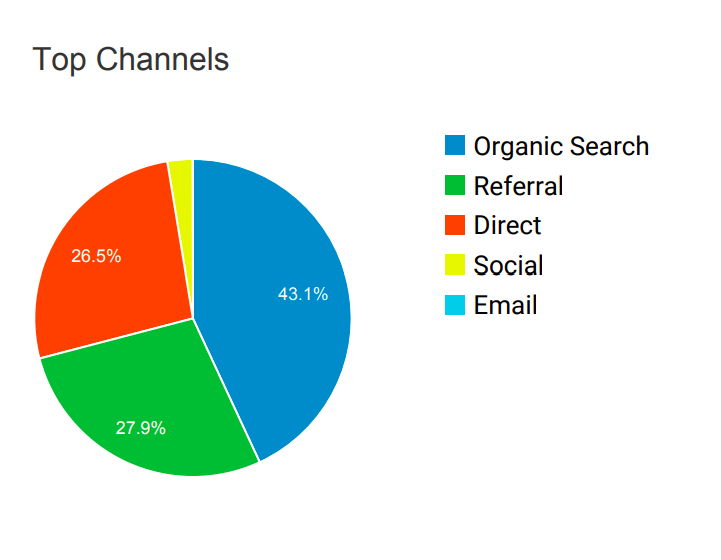
\includegraphics[width=0.5\textwidth]{vcwiz/stats/channels.png}
  \caption{User Acquisition Channels}
  \label{fig:acquisition}
\end{figure}

\subsection{Feedback}

Over the course of the months following the launch of VCWiz, we have done several surveys polling both founders and investors about their thoughts on the platform. The results of many of these surveys have already been discussed above. A few additional datapoints to highlight are that 38\% of founders surveyed spent some amount of time researching investors on VCWiz for the purpose of fundraising, and that 54\% of the founder who have \textit{not} yet used the platform for research would do so if a single feature is added (the scope of these requested features ranges from simple additions to entirely new tools). This feedback, combined with the aforementioned metrics, lead us to the conclusion that though the platform is far from finished, the current iteration has indeed provided significant value to hundreds of founders.

One piece of feedback from a founder stands out in particular, and has been reproduced below.

\begin{quote}
VCWiz was very helpful in our fundraising journey. Through it we discovered several relevant investors that weren't on our radar, and we ended up building a robust target investor list that expedited our process.
\end{quote}


\chapter{Graph Experiments}

\textbf{\#TODO: run these again}
\textbf{\#TODO: copy metrics from plots}

As part of our research into more efficiently matching founder with investors, we sought to quantitatively demonstrate some of the commonly-accepted characteristics of fundraising. Furthermore, we wish to explore how we can leverage automated ranking systems to more appropriately match companies with a source of funding. To do this, we ran various experiments on a social graph of founders, investors, and their mutual connections. This graph is built from the information provided by founders on the VCWiz platform.

As discussed in the previous chapter, one of the features of VCWiz is a CRM for founders, which integrates with their inbox and scans (the headers of) all their emails back and forth with investors registered on the platform. As part of this optional integration, founders gave permission to have their aggregate email data used for research. As we scan these emails (filtering out any irrelevant ones, as described in Listing \ref{code:parse}), we build up a graph, where each node represents an individual (using their email as a unique key), and each edge represents an email connection between two nodes. Edges are directed: there exists an edge from node $i$ to node $j$ if and only if an email has been sent from email $e_i$ to email $e_j$. Edges have weights equal to the total such number of emails sent. In order to comply with the privacy provisions made to founders, we avoided more sophisticated weighting schemes involving features extracted from the email body. These weights are ignored when doing manipulations and calculating graph metrics, unless explicitly specified.

Our motivation for modeling the underlying graph for these experiments is as follows. The majority of pre-pitch and post-pitch communication when fundraising happens over email, and almost every introduction made to an investor on behalf of a founder is done by email as well. Furthermore, emails are often sent as follow-ups to in-person meetings (at networking events, etc.). Finally, email is the preferred medium for ongoing communication between and founder and their investors. Thus, by capturing the entirety of the email graph for the subset of founders and investors on our platform, we get an accurate picture of what relationships are at play.

\section{Experiments}

The remainder of this chapter will delve into the details of several experiments. The goal of these experiments is to better identify what correlates with a successful fundraise, and how we can use this information to better match founders and investors, for the purpose of maximizing funding likelihood.

It has long been supposed that the characteristics of a founder in his or her professional network can impact, and indeed predict, how successful a fundraising attempt will be. For the purposes of these experiments, we will define success as raising at least as much money as planned, from a founder's top pick of investors, in as short a time as possible. There is lots of anecdotal evidence to support these claims\footnote{https://about.crunchbase.com/blog/fundraising-dos-and-donts/}, and recently there has been statistical evidence as well. A 2017 study uses AngelList data ``to estimate the effects of network distance in the matches resulting from Series A financing rounds'', and concludes that ``distance drives matching value and moderates preferences for experience and education''~\cite{pasquini2017matching}. We sought to verify and further elucidate this point with our graph data from VCWiz.

We would like to explore whether or not linear combinations of simple graph metrics can predict fundraising success. We first will define our metrics, and their intuitive meaning within the context of fundraising. The hypothesis is that commonly-accepted key metrics with correspond to a founder's ability to fundraise will be highly correlated with our definition of success. We will attempt to validate this hypothesis with our email graph, as well as analyze which factors are indeed the most important.

\section{Preprocessing}

Before we could analyze the graph, we had to do some preprocessing. The first step was of course to build the graph. We followed the steps in Section \ref{vcwiz:ingesting} (p. \pageref{vcwiz:ingesting}) to import each founder's emails, adding nodes and edges to a global graph as described above. Any messages skipped in the processing phase do not have their addresses added to the graph. We added several additional rules for messages to skip based on analyzing intermediate graphs for outliers (for example, nodes which had significantly higher than average in-degrees or out-degrees).

Once the graph is set up, there is one last preprocessing step that must occur. Often, there are founders who sign up for the platform, but never interact with any of the email-related features. Their nodes still get added to the graph, but are orphans that have no neighbors. These nodes can slow down metric calculations unnecessarily, and make analysis harder, so we first filter them out using the Cypher query in Listing \ref{vcwiz:cypher:orphans}.

The final step is to label each node in the graph. Every node is labeled as a \texttt{Person}, with known investors and founders being labeled as \texttt{Investor} and \texttt{Founder} respectively. These two labels are mutually exclusive. In the case a node could be labeled as both an \texttt{Investor} and \texttt{Founder}, it is treated as a investor if the person is currently employed by an institutional investment firm, and a founder otherwise.

\section{Founder Graph Analysis}

Before diving into our main experiments, we did some analysis of the basic graph that was built up in the last section. At the time of writing, the VCWiz email graph has 216,774 individual nodes, with 726 verified founders and 789 verified investors.

\subsection{Connectivity}

Looking at just the subgraph of founders who have signed up for VCWiz, we see that each node has a mean of $5.5$ neighbors, indicating that the founders on the platform often know other founder on the platform. This is consistent with the real-world behaviour of early-stage founders, who often communicate with a clique of other similar-stage founders and share resources such as tools. Indeed, it is possible that this connectivity is the result of founders spreading the word about the tool to their peers. An interesting observation here is that though these founders are not as professionally isolated as those who would benefit most from using the tool, they are perfectly set up to use the network-based functionality of VCWiz, such as Intro Paths.

\subsection{Communities}

In order to determine how much of the connectivity present is the result of founders sharing the tool with peers, we performed a connectivity analysis. If it turns out that the communities of the graph are isolated globally but strongly connected locally, it would support our hypothesis. Using Label Propagation (LPA)~\cite{2007PhRvE..76c6106R}, we can section the graph into partitions by flooding the nodes with labels: assigning each node an initial label and propagating these labels with a set of rules until distinct communities evolve.

Upon partitioning the founder graph, we find that there are 584 communities, with an average of 1.2 founders per community. Our model of the founder community on the platform was not accurate; it is not the case that there are isolated pockets of founders who are spreading news of the product to each other. Indeed, it seems that the majority of the founders on the platform are all part of a larger, loosely-defined community that cannot easily be partitioned.

An interesting finding is that the few most-populous communities are easily recognizable, after which there is a long tail of independent communities with only one or two founders. The three top communities found by LPA are Dorm Room Fund Partners, Dorm Room Fund Portfolio Companies, and YCombinator Portfolio Companies. Given that both of these organizations helped influence this work, it is not surprising to find these communities.

We also ran an alternative connectivity analysis, using the Louvain Method~\cite{2008JSMTE..10..008B}. This revealed another significant community of founders: Student Founders at UC Berkeley. However, the remainder of the communities still appear to be insignificant.

\subsection{Propensity to Investors}

We sought to answer the question of whether or not the community and neighborhood of a founder's node can predict their propensity to engage with certain investors. However, using graph structure alone, we lack sufficient signal to predict anything. We will later revisit this question, taking into account additional node metrics and founder characteristics.

\subsection{Patterns}

The profile data collected by VCWiz, when joined with the founder's email history, offers a unique opportunity to validate commonly-held assumptions in venture. We test a few of these hypotheses below.

\subsubsection{Email Volume}

The classic pattern of communication when fundraising is as follows. At the start, the founder has a very high frequency of outgoing emails, as they reach out to and/or get introductions to investors. At this stage, the founder is fighting to stay relevant, and will be following up often. Once the investors show interest and begin engaging the founder, the majority of communication happens over phone calls and in-person pitches, resulting in a decreased email volume. Finally, as the round begins to close and investors begin to commit, we expect email volume to increase again, reaching a peak as the founder pushes for final decisions and coordinates acquiring the funds.

We can test this by plotting weekly email volume over the percentage of ``committed investors'' (investors who have decided to make an investment). For email volume, we specifically use the percentage of the total emails sent during the fundraise that were sent in the given week. Fitting a third-degree polynomial to this data should show a relatively high volume to start, a sharp decline as a few investors commit, and a gradual increase as the fraction of decided investors approaches $1$.

As show in Figure \ref{fig:patterns:email}, we see a similar pattern, but not exactly what was expected. The volume of emails sent in the early stages of the round are not as high as we believed them to be, indicating there are minimal emails back-and-forth while the first investors are diligencing and deliberating over a company. Additionally, the email volume peaks when around 70\% of the investors are committed. Our best explanation for this is that the majority of the coordination around closing the round happens with the lead investor(s), including clarification and negotiation of the fine points. Following this, the remaining investors largely fall in line without much delay. We believe founders are engaging in these discussion with the lead(s) before all the investors have committed.

\begin{figure}[ht]
  \centering
  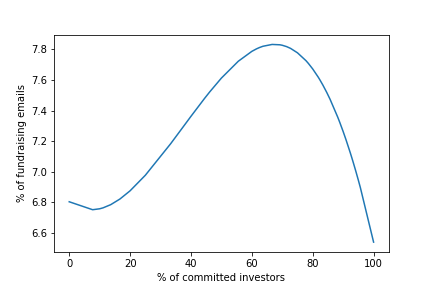
\includegraphics[width=\textwidth]{founder_rank/email_over_decided.png}
  \caption{Weekly Email Volume over \% Comitted Investors}
  \label{fig:patterns:email}
\end{figure}

\section{Baseline Ranking}

In order to evaluate any future scoring functions, we need a baseline to compare against. In the absence of a quantitative baseline scoring function, we hand-crafted a baseline ranking, incorporating our knowledge of venture capital, and the results of the research cited thus far. The goal of this baseline is to rank founders based on how likely they are to raise the largest round in the shortest period of time. We will briefly document the process of exploring features for this baseline before defining the actual scoring function.

\subsection{Potential Features}

Below are the features that were considered for the function, and our evaluation of each one for inclusion.

\subsubsection{Total funding of current round}

When available, the total amount of money raised in the current round is an excellent indicator of fundraising success, as it is normally the goal of the founder to raise as much money as possible, up to some internal maximum. This metric should definitely be included in the scoring function. Unfortunately, for many founders on the platform who are currently attempting to raise their seed rounds of funding, there might not yet be any money raised.

\subsubsection{Total funding of previous rounds}

As referenced earlier in Section \ref{chap3:tool} (p. \pageref{chap3:tool}), the First Round Capital 10 Year Project \cite{first-round-10-years} indicated much higher fundraising success rates for repeat founders. In this case, having raised money either in a previous round for the same company, or for a previous company, would give a founder the credibility and experience necessary to improve their chances for their current fundraise. We experimented including both this number, when available, as well as a binary feature indicating that this number is nonzero. Ultimately, we decided to use the raw number, as variations in this metric are significant.

\textbf{TODO: weight by average round size for the industry}

\subsubsection{Number of intro requests accepted}

While it would be useful to include a metric capturing a founder's success rate when requesting cold introductions on the VCWiz platform, there is simply not enough information for the metric we report to be indicative of anything. This follows from our earlier analysis (Section \ref{chap4:introrequests}) on why this feature saw very little usage.

\subsubsection{Number of interested investors}

A metric which is indicative of global investor interest in a company is the number of investors who have exchanged multiple emails with the founder during the timeframe of the raise. While these investors may or may not end up investing, the fact that they were interested enough to email several times is a strong signal that the founder will have options to select from when it comes time to close the round.

\subsubsection{Fraction of investors who respond}

A similar metric to the last is the percentage of investors who have emailed a founder back after the founder has initiated contact with them (either directly or through an introduction). A high value here indicates that the founder and their company are compelling enough to garner investor interest, and will have several options to select from when fundraising is over. It's also indicative of a founder's ability to reach out to investors who are a good fit for the startup.

\textbf{TODO: consider splitting cold outreach vs warm into}

\subsubsection{Average response time per investor}

The average time an investor takes to respond to a founder's email would be indicative of the investor's excitement for the founder, if all such communication happened over email and was captured by the platform. However, many founders are not using the email integrations of VCWiz, and many more will have the most crucial conversations by phone or in-person. This can create outliers which heavily skew the average and add a burdensome level of noise. Thus, this feature will not be included.

\subsubsection{Length of fundraising period}

A strong fundraise (based on our earlier criteria) is one which results in sufficient dollars being raised, in the shortest amount of time possible. Thus, the amount of time spent fundraising should be a high-signal feature: a short fundraise alone is not indicative of success, but assuming success, shorter fundraise times are better.

% Unfortunately, we observed a pattern of utilization which makes this feature problematic. As founders reach the stage of their fundraising where they are pitching venture firms and finalizing the details of the deal, they often stop using the VCWiz platform, as they are now working with a sufficiently small number of investors. Furthermore, much of the communication happens over non-email channels, as shown in Figure \ref{fig:patterns:email}. As a result, it is very difficult for us to estimate when a fundraise is over, and we do not have accurate data for this feature.

\textbf{TODO: use this feature?}

\subsubsection{Average sentiment of investors}

Intuitively, a high positive sentiment from an investor in an email is one feature of many that indicates an affinity, and a strong relationship. Looking at the data on VCWiz, strong sentiment is often associated with a pre-existing relationship, often from a previous company. Thus, while it is a noisy source of data, it should be included in our ranking function.

\textbf{TODO: plot, across all founders who raised on the platform, average sentiment of incoming emails vs total money raised}

\textbf{TODO: plot, across all founders who raised on the platform, average sentiment of incoming emails vs number of interested featured investors}

\textbf{TODO: consider normalizing against average sentiment of each investor globally}

\textbf{TODO: maybe don't use this one?}

\subsection{Evaluation}

After evaluating each of the above metrics, we drew the following conclusions. The best metric, when available, is the aggregate funding the founder has raised to date, across any company. This is the sum of the two funding-related features above. Following this, average sentiment is a good proxy for founders who have raised no money but are actively engaged in conversations. The number of interested investors is also a good proxy during the fundraise, as it represents absolute interest. The email outreach success rate (fraction of investors who respond) tends to be too noisy, as it is skewed by high-profile founders who send a very small number of emails, to already-established connections. However, the number of investors who respond after being added to a wishlist on VCWiz is a very strong signal, as it indicates no prior relationship.

\subsection{Ranking Function}

To create a ranking function from these features, we calculate a weighted sum of sort indexes for each founder, and use the position of this score in the list of all scores as the rank. We use ranks, not absolute values, across features to account for differences in scale.

We demonstrate the scoring function in Equation \ref{eq:baseline}, where $S_{m, f}$ gives the sort index for founder $f$ when the founders are sorted by metric $m$, and $W$ is the set of (metric, weight) pairs. The final ordering of the baseline is the set of founders, sorted by this score, in ascending order (a lower score represents a higher-ranked founder).

\begin{equation}
\label{eq:baseline}
  score(f) := \sum_{(m, w) \in F} S_{m, f} * w
\end{equation}

\noindent The weights we use are found in Figure \ref{fig:nfr:baseline:weights}.

\begin{figure}[ht]
\begin{tabular}{c | c}
\textbf{Feature}           & \textbf{Weight} \\\hline
Aggregate Funding          & 4 \\\hline
Average Inbound Sentiment  & 3 \\\hline
\# Responded From Waitlist & 2 \\\hline
\# Interested              & 1.5
\end{tabular}
\centering
\caption{Baseline Weights}
\label{fig:nfr:baseline:weights}
\end{figure}

This baseline, while not defensible as a ground-truth ranking for rigorous statistics, is built on sane assumptions about fundraising and venture capital. Random sampling indicates that the results are aligned with expert expectations. We will use this baseline to compare and evaluate our numerical methods for ranking, but acknowledge that it is not a perfect ranking according to the criteria we defined.

\section{Evaluation Criteria}

The next step is to define how to evaluate other ranking functions against our baseline. There are many options for evaluating ranking functions. We will discuss the options before justifying our selection. For mathematical definitions of each evaluation metric independent of our use case, we refer the reader to Section 3.2 of \cite{DBLP:journals/corr/abs-0704-3359}. These ranking functions are often used to score a permutation $\pi$ of documents given a document-set, query tuple $(D, q)$. In this case, we assume $q$ is the fixed query of founders which are most likely to succeed at fundraising, and $D$ is our list of founders.

In selecting the evaluation criteria, we imagine two relevant use-cases for our ranking functions. The first is to display a sorted list of founders to an interested party, such as an investor. The second is to use this ranking as a feature in a later process, such as enhanced matching between founders and investors (which we will explore in the next chapter).

Winner Takes All (WTA) and Mean Reciprocal Rank (MRR) are often used when displaying results based on a ranking, but both assume there is only \textit{one} top-ranked document. This does not align with either of our uses cases, so we discard them.

Discounted Cumulative Gain (DCG) takes the sum of \textit{relevances} of each founder in the ranked list (where the relevance in our case is $N - r$, with $N$ being the total number of founders, and $r$ being the rank of that founder in the baseline), weighting each founder by how early it appears in the list. We therefore get a score which increases as we put the highest-ranked founders near the start of the list, but penalizes incorrect ordering of later founders less and less. In other words, this is a metric of relative regret. This aligns well with our first use case, and provides some useful, though imperfect, information for our second.

Normalized Discounted Cumulative Gain (NDCG) simply normalizes the DCG against the number of founders in the list, so the metric can be compared across lists of different size.

Precision@n is another metric which gives preference to the top results, in this case explicitly only considering the top $n$. This metric is simply the fraction of founders in the top $n$ results that are also in the top $n$ founders of the baseline. It is a quick, useful way of evaluating a ranking for our first use case.

Root-Mean-Square Error (RMSE) is a very common error function for recommender systems (\cite{Cremonesi:2010:PRA:1864708.1864721})) which measures the differences (errors) in ranking for every founder in the list. It works very well for our second use case.

Mean Absolute Error (MAE) is another common error function, which measures the average absolute distance between a ranking and the ranking of the baseline.

Kendall's rank correlation coefficient ($\tau$) measures the ordinal association between the two lists of founders, and is often used to report on the correlation between to rankings. It roughly measures the agreement in rank over all pairs of items.

Spearman's rank correlation coefficient ($\rho$) is another measure of rank correlation. It measures the direction of association in rank between the two lists of founders.

We decided to use NDCG, Precision@n (for various values of $n$) for evaluating the quality of the rankings for the purposes of recommendation, $\tau$ and $\rho$ for calculating the rank correlation with the baseline, and RMSE and MAE for scoring the ranking as a feature to later processes. Figure \ref{fig:evaluation:formulas} shows the formulas we use for each, where $N$ is the number of founders in the list, $B$ is the baseline, $X$ is the ranking being evaluated, $R_i$ is the founder in the $i$-th position of ranking $R$, $\text{rg}(f)$ gives the rank of founder $f$ in the baseline, and $\text{sc}(R, f)$ gives the \textit{score} of founder $f$ under ranking $R$. Each ranking that we will be evaluating has a scoring function, which is in the range $[0, 1]$ for each founder. For the baseline, we assign scores by simply scaling the rank to be in this range.

\begin{figure}[ht]
\begin{equation}
  \begin{array}{c >{$\displaystyle}Sc<{$}}
    \text{\textbf{Metric}} & \text{\textbf{Formula}} \\
    \text{DCG}(X) & \sum_{i=1}^{N} \frac{2^{N - \text{rg}(X_i)} - 1}{\log_2{i + 1}} \\
    \text{NDCG}(X) & \frac{\text{DCG}(X)}{\text{DCG}(B)} \\
    \text{Precision}(X, n) & \frac{|X_{0:n} \bigcap B_{0:n}|}{n} \\
    \tau(X) & \frac{\sum_{i=1,j=1,j \neq i}^N \text{conc}(i, j, X)}{N (N - 1)} \\
    \rho(X) & 1 - \frac{6 \cdot \sum_{i=1}^N \text{drg}^2(X, B, i, i)}{N (N^2 - 1)} \\
    \text{RMSE}(X) & \sqrt{\frac{\sum_{i=1}^N \big(\text{dsc}(X, B, X_i)\big)^2}{N}} \\
    \text{MAE}(X) & \frac{\sum_{i=1}^N \big|\text{dsc}(X, B, X_i)\big|}{N}
  \end{array}
\end{equation}

\begin{align*}
 \text{drg}(X, Y, i, j) &:= \text{rg}(X_i) - \text{rg}(Y_j) \\
 \text{dsc}(X, Y, f) &:= \text{sc}(X, f) - \text{sc}(Y, f) \\
 \text{conc}(X, i, j) &:= \text{sign}\big(\text{drg}(X, X, i, j)\big) \cdot \text{sign}\big(\text{drg}(B, B, i, j)\big)
\end{align*}

\centering
\caption{Evaluation Criteria}
\label{fig:evaluation:formulas}
\end{figure}

Finally, we must define our null hypothesis, so that we can provide p-values for our rank correlations. In this case, the null hypothesis is that the correlation between the baseline and the ranking in question is 0. Thus, p gives the probability that the two uncorrelated rankings would give them same rank correlation metric value.

\section{FounderRank}

We will be ranking founders based on the information we collected on the VCWiz platform. We wish to score nodes based on graph metrics in an email graph of fundraising relationships. To do this, we first need to define a single scoring function which captures our goals. Thus we introduce FounderRank.

FounderRank is a metric in the range $[0, 1]$ that quickly communicates the strength of a founder in the global fundraising graph of founders, investors, and their mutual connections (i.e. the VCWiz Email Graph). A strong node is able to rapidly spread the word about their startup, start conversations with relevant and desirable investors, and convince investors to invest in them. These abilities are crucial for fundraising, which is in turn crucial for the survival of a startup.

Note that we are currently evaluating how well a founder can fundraise conditioned on them knowing who they would like to fundraise from. We are not tackling the issue of discovering investors, which we have touched on in the previous chapter, and will explore further in the next.

\subsection{Core Characteristics}

A combination of existing studies and our own interviews with numerous seed-stage firms reveals three intuitive properties of a founder's node in a professional or social graph which are desirable when fundraising: \textbf{importance}, \textbf{influence}, and \textbf{access}. Note that these characteristics do not take into account factors such as domain expertise, personality, and pedigree, all of which will also contribute to a successful fundraise. We are focusing exclusively on network properties for this experiment.

The first characteristic is \textbf{importance}. Importance looks at how crucial a founder is in his or her own ecosystem. This property is important as it is indicative of the founder's degree of expertise. It has been shown that in efficient professional information networks, entrepreneurs are bounced from expert to expert until they have sufficient information to answer their query~\cite{BIRLEY1985107}. The more crucial a founder is to a domain, the more access to high-quality information he or she will have. Thus, founders who have more importance are likely to be seen as a less risky investment, increasing the chances an investor responds positively to a fundraising proposal.

The second characteristic is \textbf{influence}. Influence captures how effectively a founder can effect change in their ecosystem and solicit aid from their peers. In other words, how likely are other founders to help this founder? A study on interorganizational networks of young companies found supporting evidence to the fact that ``third parties rely on the prominence of the affiliates of those companies to make judgments about their quality''~\cite{10.2307/2666998}. Founders who have high influence can leverage this to convince investors to give them funds.

The third characteristic is \textbf{access}. This is the notion of how well a founder can get in front of the investors of their choice. The more directly connected a founder is to an arbitrary investor, the more likely that investor is to respond to an inbound request (either via an introduction or cold) for funding. Additionally, a high degree of access means a founder has many options to chose from when it comes to starting conversations with investors. This follows from the more general finding that proximity in a graph to providers of valuable resources gives a node access to many viable alternatives\cite{10.2307/3069443}. This can be valuable when a founder's top choice of investor does not work out, which is often the case.

\subsection{Graph Metrics}

To quantitatively evaluate the impact of each of these characteristics, and measure their predictive capability, we need to find graph metrics which correspond to each.

For \textbf{importance}, we selected PageRank~\cite{page1999pagerank}, the canonical starting point for ranking nodes in graphs. PageRank recursively evaluates node importance by analyzing the importance of nodes which link to the node in question. It is a widely-accepted measure of node importance. We use a normalized PageRank~\cite{berberich2007comparing}, which accounts for the number of nodes and structure of the graph.

For \textbf{influence}, we selected Betweenness Centrality~\cite{10.2307/3033543}. Betweenness Centrality is the count of the number of shortest paths (over all pairs of nodes) that pass through the node in question. The rationale is that if a node is on the intro path for a pair of people, that node has influence over that pair, as it can control whether or not the introduction is made. This makes the assumption that every communication request goes along the shortest path, which is not perfectly accurate, but is sufficient for our purposes.

For \textbf{access}, we selected Closeness Centrality~\cite{FREEMAN1978215}. The Closeness Centrality of a node is inversely proportional to the node's distance from every other node. Thus, this metric measures how ``close'' a node is to the other nodes in the graph, based on shortest-path lengths, normalized for the number of nodes in the graph. The rationale is that if a node can access every other node in the graph, on average, via a short path, the node must have better access than a node that must use longer paths. Once again, this assumes that the length of the shortest path between nodes is the determiner of connection strength. Based on the data presented and cited thus fair, this is a fair assumption.

To use these metrics, we take the pre-processed graph above, and calculate the raw metric value for each node. We then normalize it as specified above, and finally scale it to be in the range $[0, 1]$. We now have a number which represents the metric for a node, relative to the other nodes in the graph, and on a standard scale. Note that we do not yet specify how to combine these metrics, we are simply calculating them.

\subsection{Naive FounderRank}

We now begin to explore ways to combine these three selected graph metric to produce a scoring function that we can compare against our baseline. The Naive FounderRank (NFR) method simply averages these three numbers, per node, to arrive at a score in $[0, 1]$.

\subsubsection{Random Model}

In order to have a model to compare against, we first start with a random model, which simply generates a score randomly and uniformly in $[0, 1]$ for each founder, then ranks them based on this score. The metrics for our random model are found in Figure \ref{fig:rand:results}.

While the random model would never be used for a serious application, it is worth noting that this way of sorting founders is not too far from the techniques used by many analysts in the real world today. The status quo at many firms involves haphazardly picking new companies to investigate based on ``gut feelings'': heuristics based on pattern-matching previous successes without any grounding in data. In one extreme case, an individual we interviewed claimed he triages companies by first sorting them alphabetically.

\begin{figure}[ht]
\begin{tabular}{c | c | c | c | c | c | c | c}
NDCG & P@5 & P@10 & P@20 & $\tau$ & $\rho$ & RMSE & MAE  \\
0.270 & 0.2 & 0.1 & 0.05 & 0.00689 & 0.0100 & 0.255 & 0.234 \\
\end{tabular}
\centering
\caption{Random Results}
\label{fig:rand:results}
\end{figure}

$\rho$ and $\tau$ have p-values of $0.808$ and $0.813$ respectively. As expected, there is essentially no correlation between the random model and the baseline.

\subsubsection{Evaluating NFR}
\label{ch5:nfr:eval}

We now move on to evaluating NFR. The first observation we made when trying to rank the founders based on NFR is that our rankings totally missed founders on the platform who are not currently fundraising, but who are known to be repeat founders who have successfully fundraised in the past. This was a result of our email graph only spanning the last year. Relationships in the venture capital world take years to build up, and we were not evaluating them over a large enough timeframe. Thus, we re-built our graph to incorporate the last five years of data, which gave us a much more comprehensive view of the ecosystem.

The below observations and conclusions are all drawn from this new graph, with up to five years of email data from 558 founders.

We sorted the founders in our original list by their NFR score, and then evaluated this ranking based on our earlier-established criteria. The results are shown in Figure \ref{fig:nfr:results}.

\begin{figure}[ht]
\begin{tabular}{c | c | c | c | c | c | c | c}
NDCG & P@5 & P@10 & P@20 & $\tau$ & $\rho$ & RMSE & MAE  \\
0.448 & 0.2 & 0.3 & 0.2 & 0.484 & 0.673 & 0.0827 & 0.0637 \\
\end{tabular}
\centering
\caption{NFR Results}
\label{fig:nfr:results}
\end{figure}

The p-values for $\tau$ and $\rho$ are respectively $10^{-65}$ and $10^{-75}$.

\subsubsection{Discussion}

As expected, the naive model easily and confidently beats the random model on every metric. While this is intuitive (there must be \textit{some} information in this graph), it is important to point out that even such a simple, naive model can best a standard seen often in venture today. If the goal is to use this ranking to surface interesting founders, NFR is an acceptable solution, albeit not great. The precision is still too low to be considered truly valuable. As a feature, the rank correlation observed in NFR is impressive. The degree to which naively combining graph metrics gives a score correlated to the baseline indicates how important the founder's position in their social-professional graph is.

We can interpret $\tau$ as saying that there is reasonable agreement between the rankings presented by NFR and the baseline, and $\rho$ as saying the direction of association in the rankings is positive, and significantly so: more often than not, the ranking of NFR tends to increase when the baseline does the same.

A final observation is that, as expected, all of the relative regret metrics increased after rebuilding the graph over a longer time period. It is easier to identify strong founders when relationships over a long period of time can be taken into account. Founders in the middle of the ranking largely stayed in the same position, as no new information was revealed about them.

\subsubsection{Edge Weights}

One interesting experiment we considered was using the frequency of emails exchanged between two nodes as an edge weight. Running the same metric algorithms on this new weighted graph should render even more accurate data about relationships, the position of a given node, and therefore the strength of the founder in the graph. Unfortunately, there is a significant amount of work involved in re-writing the metric algorithms to incorporate edge weights, and we did not have the time to explore this. We leave it as future high-potential work.

\subsection{Weighted FounderRank}

The next model we experimented with is a linear combination of the three graph metrics, as determined by a simple linear regression, using the hand-crafted baseline ranking as labels. We fit a standard linear regression model to the baseline ranking, using each of the three graph metrics as a feature. We get an $R^2$ value of $0.39$, with evaluation metrics as shown in Figure \ref{fig:wfr:results}. The change in metrics is negligible, with NDCG, $\tau$, and $\rho$ increasing slightly, but our error functions (RMSE and MAE) also increasing slightly.

\begin{figure}[ht]
\begin{tabular}{c | c | c | c | c | c | c | c}
NDCG & P@5 & P@10 & P@20 & $\tau$ & $\rho$ & RMSE & MAE  \\
0.449 & 0.2 & 0.3 & 0.2 & 0.490 & 0.680 & 0.103 & 0.0787 \\
\end{tabular}
\centering
\caption{WFR Results}
\label{fig:wfr:results}
\end{figure}

More interestingly, we can examine the effect on our evaluation metrics and $R^2$ by using different combinations of the three graph metrics, with the goal of determining their relative importance.

\subsubsection{Sole Metrics}

If we rank our founders based solely on their PageRank, we get abysmal evaluation metrics, with the exception of NDCG, which is significantly higher at $0.527$. This implies that if our sole concern was surfacing the best few founders from the batch, sorting by PageRank would be a good option. This corroborates our conclusions from extending the timeframe over which the graph is built: the best founders often are well-embedded and have built up strong relationships over years, giving them a high PageRank.

If we rank solely based on a founder's betweenness, every metric is strictly worse. The $R^2$ value of the regression actually goes negative, indicating that this metric alone is a very poor model of a founder's potential for fundraising success. Furthermore, a founder's betweenness is highly correlated with their PageRank (a Pearson correlation coefficient of $0.913$), making it unnecessary to ever consider it.

Finally, if we rank solely on closeness, we end up with a lower NDCG (at $0.375$), but increased P@5 ($0.4$) and $\tau$ ($0.498$). The RMSE increases to $0.135$. The conclusion here is that how much access a founder has in the graph can offer a marginally better ranking in isolation, though at the cost of less accurate individual scores. For ranking, it appears that closeness explains more of the optimal ranking than any other metric, and this is supported by the relatively close $R^2$ value of $0.348$. While it is far from a perfect model, a node's closeness centrality in the email graph explains about 35\% of the variance of a hand-tuned ranking of the founders in the graph.

Our conclusion from testing these individual metrics is that access is most important aspect of a founder's node in the graph, but a sufficiently high importance (PageRank) can compensate for a lower closeness centrality.

\subsubsection{Optimal Combination}

Based on the above, the optimal combination of features is some linear combination of PageRank and Closeness Centrality. We ran another linear regression with these two features, resulting in a model that has similar evaluation metrics, save for the highest NDCG seen yet ($0.533$). Adding PageRank to Closeness Centrality in our model brings $R^2$ to $0.391$, a $12.8$\% increase.

\subsubsection{Conclusion}

The goal of these experiments on the VCWiz Email Graph was to explore whether the data stored in the graph structure and relationships could improve the process of predicting a founder's ability to fundraise, for use in the founder-investor matching process by both humans and other models. We have shown that there is signal in our selected graph metrics of founder nodes.

Through these experiments, we have determined that graph metrics alone can do a good job scoring founders. The rankings are not perfect, and can only explain about 40\% of the variance seen in the baseline they are compared against, but they significantly best the status-quo of an effectively random model, and have considerable rank correlation with the baseline ($\rho = 0.680$, p $\approx 0$). Upon examining the individual graph metrics, we see that Closeness Centrality, which corresponds to a founders ``access'' in the graph, is the driving factor, with exceptions in the case of very successful founders who have extraordinary PageRank. We also find that Betweenness Centrality, which indicates a founder's influence over introductions, is a near-meaningless metric, with information that is captures almost entirely by PageRank.

The takeaway of access being a driving factor to founder fundraising success further motivates our work on the VCWiz platform. We've demonstrated that founders who have a short average distance to investors tend to see success fundraising. A stated goal of the platform is to increase founders' access to investors, a demonstrably high-impact outcome. We accomplish this by helping founders discover and understand investors who are within reach of their network, and facilitate connections which add edges in the relationship graph. VCWiz enables these connections for all founders, enshrining equality in what is otherwise an insider's game.

\section{FounderRank with Investment Data}

The next experiment explores whether the conclusions of the FounderRank experiment hold true on the global graph of venture investments. If so, we wish to explore whether adding global investment data to the VCWIz Email Graph can augment it and provide even better rankings.

We begin with considering the public graph of venture fundings, as reported by VCWiz. At the time of writing, this database contains $288,720$ founders, $92,843$ investors, and $57,131$ investments. For an overview of how this data is collected, see Section \ref{ch4:data} (\pageref{ch4:data}). The graph is constructed by creating a node for every founder and investor on the platform, each tagged as such. For each instance of an individual investor investing in a founder's company (see Section \ref{ch4:partners} for an overview of how this information is inferred), two edges are added: one from the founder to the investor, and one from the investor to the founder.

\subsection{Baseline}

As before, there is no ground-truth ranking of the founders in this graph, so we need to generate a baseline. We will focus on public metrics involving the past experience of the founders, as well as the aggregate money they have raised. We rely on the work done in \cite{2017arXiv170604229H} as justification for selecting these metrics.

\begin{quote}
We see that the top non-sector features are related to the past experience of the leadership (executive acquisition, executive IPO, advisory IPO, leadership age). The investor feature maximum acquisition fraction is also one of the top non-sector features. This suggests that companies with experienced and successful leadership and investors have increased drift which results in a higher exit probability.
\end{quote}

The features we selected are Job IPO, Job Acquired, Executive IPO, Executive Acquired, Advisory IPO, and Advisory Acquired. These features track initial public offerings and acquisitions across any company the founder has worked at, started, or advised. The specific feature we use is the sum of all these numbers. We call this feature Affiliated Exits.

Using the same process as before (a combination of manual inspection, sane priors about venture capital, and consulting experts), we arrived at the baseline weights shown in Figure \ref{fig:fri:baseline:weights}. We use the same scoring function construction as in Section \ref{ch5:nfr:eval}. We will also use the same evaluation metrics.

\begin{figure}[ht]
\begin{tabular}{c | c}
\textbf{Feature}   & \textbf{Weight} \\\hline
Affiliated Exits   & 4 \\\hline
Aggregate Funding  & 1
\end{tabular}
\centering
\caption{Baseline Weights}
\label{fig:fri:baseline:weights}
\end{figure}

The rationale for these weights follows from the metrics from \cite{2017arXiv170604229H} which have been shown to correlate with a founder's success rate, including ability to successfully fundraise. We additionally add the Aggregate Funding feature from the last experiment, to acknowledge that founders who have raised a large amount of capital in the past are more likely to be trusted as stewards of capital in the future.

One interesting observation about this baseline is that rewarding a large number of exists gives us a ranking that surfaces many founders who are now investors. This aligns well with career paths seen in the venture world: founders who take a company from birth to exit have experience that is highly sought-after in investors.

\subsection{Random Model}

Much as before, a random model shows the expected characteristics with all our evaluation criteria. There is no rank correlation with the baseline.

\subsection{Optimal FR+I Model}

The best linear combination of graph metrics for the global funding graph tells a very different story than that of the VCWiz Email Graph. In this case betweenness, which we previously identified as a near-useless metric, has a large negative coefficient when included, with a model that is effectively the same as omitting it altogether. The remaining combination of PageRank and closeness still gives us an abysmal result: an $R^2$ of $-0.268$, with a $\rho$ of $0.192$ (with a p-value of effectively $0$). We see that there is no way to give a reasonably good ranking function based on these three graph metrics on the graph of venture fundings, implying that this graph carries very different information from the social-professional email graph.

\subsection{Broader Venture Ecosystem}

We further experimented with the graph of funding data, augmenting it with data about both co-founding relationships (founder-founder) and co-investing relationships (investor-investor). The co-investing relationships (an edge between a pair of investors if and only if those two investors have participated in the same funding round of a company) did not significantly improve our models, but the co-founding relationships did.

In this new graph of investment and co-founding relationships, the best model is the one that solely uses the closeness metric. This is consistent with all our previous conclusions. With this model, we get a $\rho$ of $0.357$. While this is not as strong a correlation as the email graph was, it still shows a similar result. This result is consistent, as we expect there to be less information in a graph of public investment and cofounding data than there is in a social-professional graph that reveals the many conversations which do not end in an investment or new company.

\subsection{FR+I with Email Data}

We have shown so far that the data in the global funding graph alone is not sufficient to show any meaningful correlation. However, we know that the private email graphs of founders \textit{do} have predictive power. To explore whether or not there is any value in the global funding graph's relationships in the context of ranking founders, we took the VCWiz Email Graph and overlaid the graph of investment and co-founding relationships from the previous section.

The results confirm what we expected: the email graph contains sufficient information to predict a founder's fundraising ability, and given this, the public funding graph adds information which makes increases the correlation of the model's ranking with the baseline. Upon adding the public graph nodes and relationships, we see an increase in $\rho$ from $0.680$ to $0.695$, and a doubled P@5 of $0.4$.

\subsection{Conclusion}

Our conclusion from the above experiments is that the public graph of venture funding relationships does not provide adequate information on social-professional networks to draw conclusions about the strength of a founder (and his or her ability to fundraise). While private graphs, such as the VCWiz Email Graph, which capture \textit{all} communication between founders, investors, and their intermediaries can be useful in evaluating and characterizing founders, public data falls short. We believe this is in part due to private conversations including those which do not culminate in a fundraising relationship; while an investor may not invest in a founder, a strong relationship might still exist which can be leveraged at a later date. Furthermore, public data makes it difficult to infer social friendships which are captured in emails, and might be crucial to introductions. This public data can, however, still be used to successfully augment an existing private graph with additional relationships from venture investments past and present. Since the public graph adds relevant relationships to those implied by emails, we see an increase in the efficacy of the email-based graph when augmenting it with the global funding graph.

\section{InvestorRank}

For this final experiment, we explore the value in calculating the same graph metrics considered above for the investors themselves.

\textbf{TODO: run the numbers and see if it makes sense to include, using co-investment edges}

\textbf{TODO: baseline ranking of sum of investments which have exited}
% (don't want to use exit amounts bc outliers skew everything)

% See if it makes sense to run these graph metrics for investors on the graph themselves. See is there if correlation between InvestorRank and FounderRank of the founders invested in by that investor. How to do correlation calculation for many to many -- Pairwise?

% Future: Given that the FounderRank metric seems indicative of a founder's ability to raise, and that raising is a crucial part of keeping a company alive, does ranking investors by the mean founder rank of the founders they've invested in give us a reasonable ranking of investors? Manually inspect it, also compare it to baseline, which can use features like \# of exists, total follow-on raised, and total valuation at IPO sum.


\chapter{Conclusion}

\section{Summary of Contributions}

In this thesis, we have presented two major contributions. The first is VCWiz, a tool which aspires to aid founders in finding and connecting with seed investors. The second is a series of experiments centered around FounderRank, a method of ranking founders based on their likelihood of a successful fundraise.

\subsection{VCWiz}

Through the process of designing and implementing VCWiz, we identified and enumerated three major areas, each with several opportunities, where software tools could improve the investor-founder matching process. We surveyed a group of seed-stage founders and discovered that existing tools for investor discover, research, and outreach were isolated, lacking in functionality, or not practical to use. To address this, we built three iterations of a holistic fundraising tool.

The first iteration of the tool revealed the high bar for functionality and ease of use when it comes to replacing household tools like spreadsheets. The second iteration's feedback focused on the need for a platform to be comprehensive and customizable. The third iteration, which is currently live and in use by hundreds of founders, has proven that there are opportunities to make early-stage investing easier and more manageable to a diverse range of startup founders. The feedback and data from this tool have shown that VCWiz does indeed accomplish its goals of making fundraising more efficient, and more accessible. Hundreds of founders, amongst them many underrepresented minorities, have successfully used the VCWiz platform to discover new investors, leverage their networks, and raise a round of financing.

The VCWiz Email Graph, collected from the founders on the platform, serves as the basis for the study described in this thesis.

\subsection{FounderRank}

Using the VCWiz Email Graph, we explored the structure and interactions of a graph of seed-stage founders from a variety of backgrounds and pedigrees. We identified that there are three important social characteristics of a founder when fundraising: importance, influence, and access. We identified three graph metrics that correspond to the three characteristics: PageRank, Betweenness Centrality, and Closeness Centrality.

With a linear regression, we showed that the optimal linear combination of these three graph metrics can explain about 40\% of the variance found in a hand-crafted baseline ranking of founders, with a rank correlation of $0.68$. Furthermore, we identified access as the most important characteristic a founder can have when fundraising, followed by their importance. Influence, as proxied by Betweenness Centrality, has a near-perfect correlation with importance, and provides very little information when ranking founders.

By running similar processes over the graph of public funding data, we discovered that there is not sufficient information in the relationships of venture investments alone to predict fundraising success. However, this graph does contain information which can better inform rankings of founders when used to augment a social graph such as the VCWiz Email Graph. Doing so increases the rank correlation defined above non-trivially.

\textbf{TODO: summarize other experiments as we finish them}

\section{Future Work}

\subsection{VCWiz}

\subsubsection{Requested Features}

On the VCWiz platform, there are several high-demand features which founders have requested repeatedly. In a survey of 118 founders, the most requested features were:

\begin{itemize}
  \item Importing and syncing intro paths from LinkedIn in addition to email
  \item Supporting Microsoft Outlook for email syncing
  \item Per-investor notes across communities of founders
  \item Shared accounts for co-founders to share
  \item A faster, more responsive filtering interface
  \item Incentives for investors to respond to Intro Requests
  \item Custom CRM columns
  \item More angel investors in the database
  \item Information on why an investor made a given investment
\end{itemize}

Future work would include evaluating and implementing these features, as well as continuing to find creative data sources for aggregating more information on investors. Performance is another opportunity for future improvement: the average API request involving a filter operation takes about one second.

\subsubsection{Community Support}

One major area of exploration to consider is adding community functionality to VCWiz. Currently, the platform has no direct way for founders to contribute back information on the investors they interact with. While their usage patterns and communication history are used to inform rankings, there is an opportunity to add founder-reported attributes to investor profiles. Doing this would allow founders to learn from the aggregate knowledge of their peers, without having to undertake a laborious set of meetings and phone calls. Examples of this include personality traits of investors, investment criteria, and evaluations of the extra-financial value discussed in Section \ref{ch3:motivation:research}.

We began exploring this set of features by forming a partnership with KnowYourVC\footnote{https://knowyourvc.com/}, a founder-oriented review site for venture capitalists. While founders cannot currently report their experiences directly on VCWiz, the can see reviews and tags pulled in from KnowYourVC's API.

\subsubsection{Ranking \& Filtering}

The results of our study show that there is merit to ranking founders and investors based on the information collected on the VCWiz platform. There is further opportunity to use this information in surfacing investors to founders during the discovery phase of their fundraise.

The ranking function discussed in Section \label{ch4:filtering} is currently very similar for every founder on the platform. Future work could explore further customization of this ranking, based on preferences collected from the founder. For example, finding an investor that is in the same physical location might be much more important to a founder than finding one who has deep expertise in a specific industry, or vice-versa.

\subsection{FounderRank}

While we have examined the relationship between founder and investors in social graphs, we have yet to rank and score the two sets of nodes jointly. There are several opportunities to explore the efficacy of this technique, including explicitly exploring how the scores of the founders that an investor has funded correlate with the rank of the investor, and vice-versa.

\subsubsection{Clustering}

The rank assigned to a founder (or investor) is an indicator of their social characteristics, which might make it a useful feature when clustering individuals. One hypothesis to test in the future is that investors prefer to invest in founders who have a similar relative rank to themselves. If this is true, and investors have an affinity to similarly-ranked founders, then it would be prudent to show founders investors of a comparable rank in a tool such as VCWiz, so as to maximize their chances of an investment being made.

\subsubsection{Recommender Systems}

The experiments to date with data generated from founders on VCWiz has focused on scoring and ranking founders and investors. However, there is another, related application of this data in recommender systems. The crucial hypothesis to test is that incorporating data from the platform increases the quality of recommendations over classic techniques. This information includes attention-based features, such as which investors are clicked on, reached out to, and interacted with. If this hypothesis is proven, a recommender system would increase the efficiency of investment matches, with founders discovering investors they would not have otherwise. However, we must be careful to not sacrifice the equity of our system: as discussed in Section \label{ch2:matching}, models trained on existing data can incorporate the dangerous biases that are pervasive in venture capital.

One could test this hypothesis by beginning with a classic item-based recommender system, trained on features extracted from the investor's profile, as well as InvestorRank. This model could be evaluated against a simple baseline, which suggests the co-investors of a startup's competitors as the recommended investors. The performance of this model could then be compared against a hybrid model, which adds a user-based layer that is trained on the click and outreach data of founders on the VCWiz platform.

\chapter{Conclusion}

\appendix
\chapter{VCWiz Queries}

\begin{lstlisting}[frame=single,language=SQL,basicstyle=\footnotesize,columns=fullflexible,label={vcwiz:sql:query},caption={Firm Filter Query}]
SELECT
  subquery.*,
  firm_partners.partners AS partners,
  firm_recent_investments.recent_investments AS recent_investments,
  firm_coinvestors.coinvestors AS coinvestors
FROM (
  SELECT
    distincted.*,
    firm_velocities.velocity
  FROM (
    SELECT
      DISTINCT ON (fullquery.id) fullquery.*
    FROM (
      SELECT
        firms.*,
        wo.rn
      FROM (
        SELECT
          subquery.id,
          row_number()
          OVER (
          ORDER BY
            subquery.ti_sum DESC,
            subquery.c_cnt DESC) AS rn
        FROM (
          SELECT
            firms.id,
            SUM(COALESCE(firm_investor_aggs.target_count, $1)) AS ti_sum,
            COUNT(DISTINCT companies.id) FILTER (
              WHERE companies.location = $2
            ) AS c_cnt
          FROM
            firms
            INNER JOIN investments ON investments.firm_id = firms.id
            INNER JOIN companies ON companies.id = investments.company_id
            INNER JOIN firm_investor_aggs ON firm_investor_aggs.firm_id = firms.id
          WHERE (
            firms.id IN (
              (
                  SELECT
                    firms.id
                  FROM
                    firms
                  WHERE (firms.location && $3)
              )
              UNION
              ::~ (
                SELECT
                  firms.id
                FROM
                  firms
                  INNER JOIN investments ON investments.firm_id = firms.id
                  INNER JOIN companies ON companies.id = investments.company_id
                WHERE (companies.location = $4)
              )
            )
          )
          GROUP BY
            firms.id
          ORDER BY
            ti_sum DESC,
            c_cnt DESC
          LIMIT $5
        ) AS subquery
        LIMIT $6
      ) AS wo
      INNER JOIN firms
      USING (id)
    ) AS fullquery
  ) AS distincted
  LEFT OUTER JOIN firm_velocities ON firm_velocities.firm_id = distincted.id
ORDER BY
  rn OFFSET $7
LIMIT $8) AS subquery
  INNER JOIN firm_recent_investments ON firm_recent_investments.firm_id = subquery.id
  INNER JOIN firm_coinvestors ON firm_coinvestors.firm_id = subquery.id
  INNER JOIN firm_partners ON firm_partners.firm_id = subquery.id
\end{lstlisting}

\newpage

\begin{lstlisting}[frame=single,language=SQL,basicstyle=\footnotesize,columns=fullflexible,label={vcwiz:sql:view},caption={Denormalization of Individual Investor Properties}]
SELECT
  firms.id AS firm_id,
  COALESCE(SUM(investors.target_investors_count), 0) AS target_count,
  bool_or(COALESCE(investors.featured, false)) AS featured,
  bool_or(COALESCE(investors.verified, false)) AS verified
FROM firms
  INNER JOIN investors ON investors.firm_id = firms.id
GROUP BY firms.id
\end{lstlisting}

\begin{lstlisting}[frame=single,basicstyle=\footnotesize,columns=fullflexible,caption={Intro Paths},label={vcwiz:cypher:intro}]
MATCH (other:Investor), path = shortestPath((me)-[*1..4]-(other))
WHERE id(me) = {founder_neo_id} AND id(other) = {investor_neo_id}
RETURN path, reduce(count = 0, r IN relationships(path) | count + coalesce(r.count, 0)) AS total
ORDER BY total DESC
LIMIT 3;
\end{lstlisting}

\clearpage
\newpage

\chapter{VCWiz Data Models}

These Entity-Relationship diagrams are generated with rails-erd\footnote{https://github.com/voormedia/rails-erd}.

\begin{figure}
  \includegraphics[width=\textwidth]{vcwiz/models/hierarchy.pdf}
  \caption{VCWiz Model Hierarchy}
  \label{vcwiz:model:hierarchy}
  \centering
\end{figure}

\begin{figure}
  \includegraphics[width=\textwidth]{vcwiz/models/content.pdf}
  \caption{VCWiz Models}
  \label{vcwiz:model:content}
  \centering
\end{figure}

\clearpage
\newpage

\chapter{VCWiz Routes}

\begin{figure}[h]
\caption{Frontend Routes}
\label{vcwiz:routes:frontend}
\begin{multicols}{2}
\begin{verbatim}
/login
/logout
/signup

/discover
/outreach
/filter
/search

/privacy
/terms
/founders/unsubscribe(/:token)

/firm/:id(/:slug)
/investor/:id(/:slug)
/company/:id(/:slug)
/list/:list(/:key/:value)
\end{verbatim}
\end{multicols}
\end{figure}

\begin{figure}[h]
\caption{Investor Routes}
\label{vcwiz:routes:investors}
\begin{multicols}{2}
\begin{verbatim}
/investors/token/:token
/investors/signup
/investors/settings
/investors/contacts
/investors/update_contacts

/intro/opt_in
/intro/decide
/intro/pixel/:token.png
\end{verbatim}
\end{multicols}
\end{figure}

\newpage

\begin{figure}[h]
\caption{Internal API Routes}
\label{vcwiz:routes:api}
\begin{multicols}{2}
\begin{verbatim}
/api/intros/:id/preview
/api/intros/:id/confirm
/api/intros
/api/intros/:id
/api/investors/:id/interactions
/api/investors/:id/intro_paths
/api/investors/:id/verify
/api/investors/filter
/api/investors/search
/api/investors/fuzzy_search
/api/investors/entities
/api/investors/recommendations
/api/investors/locations
/api/investors/add
/api/investors
/api/investors/new
/api/investors/:id/edit
/api/investors/:id
/api/companies/search
/api/companies/query
/api/companies/:id
/api/firms/:id/intro_paths
/api/firms/filter
/api/firms/filter_count
/api/firms/locations
/api/firms/intro_path_counts
/api/firms/lists
/api/firms/list/:list(/:key/:value)
/api/firms/:id
/api/message/open
/api/message/click
/api/message/bounce
/api/message/unsubscribe
/api/message/demo
/api/message
/api/pubsub/generation
/api/target_investors/import
/api/target_investors/bulk_import
/api/target_investors/poll/:id
/api/target_investors
/api/target_investors/new
/api/target_investors/:id/edit
/api/target_investors/:id
/api/founder/disable_scanner
/api/founder/event
/api/founder/locations
/api/founder
\end{verbatim}
\end{multicols}
\end{figure}

\clearpage
\newpage

\chapter{Potential Products}
\label{intro:products}

We have spent time exploring possible tools that could be built to aid in various stages of the venture pipeline. Each tool is identified below, along with the motivation and a brief summary of the technical challenges involved.

\section{Sourcing}

We have identified two opportunities to do with sourcing, both on the outbound flow side.

\subsubsection{A system to aggregate signals from founders and predict the intent to start a company}

Founders often emit signals that indicate they are starting a new company, often long before they officially announce their new endeavor. These signals can be explicit (changing a job title on LinkedIn, or biography line on Twitter) or implicit (leaving a job, moving cities, or attending entrepreneurial events). In isolation, these signals are not strong, but in aggregate they can be strongly correlated with the intent to start a company.

We see an opportunity for a system that monitors the social networks of a GP, identifying and aggregating potential signals. The technical challenges include linking seemingly-unrelated signals across networks and schemas, and inventing a ranking algorithm which can present the most likely potential founders given a set of signals. We would likely use these signals as machine learning features.

\subsubsection{A system to discover and monitor promising out-of-network individuals and organizations}

While there are a plethora of announcements and releases online which would indicate an investment-worth company has formed, humans are not capable of monitoring and filtering the wealth of information generated on the internet on an ongoing basis. Thus, a GP's sourcing abilities are largely limited to the founders they can discover in their network.

We propose a system which treats the relevant information on the Internet as a connected, directed graph, which can be monitored and have its nodes ranked (as PageRank does for search engines). Every interesting community (such as educational institutions) could have its own independent graph, and the top-ranked nodes of each graph could be surfaced for easy human review. The technical challenges around this system include a lack of labeled training data (what constitutes an ``interesting'' node?) and the noisiness of the web (there are many sites linked from a community that contain irrelevant or even misleading information).

\section{Analyzing}

When is comes to analyzing, there are two major project proposal we considered.

\subsubsection{A system to filter, categorize, and rank the companies in a venture pipeline}

Many seed-stage funds suffer today from an overwhelming pipeline of startup companies to consider. There is considerable data available on these companies which seems to be correlated to how investment-worthy the company is at first glance. At the very least, the cheap filters applied by investors are mimicable through existing data (alma maters of founders, size of initial market, sentiment of partners after first meeting).

We propose a system which uses the information associated with pipeline companies to categorize each company into buckets that predict how far in the pipeline the company will move, using these buckets to filter and prioritize the pipeline. This will be an online, semi-supervised clustering problem which receives constant feedback from partners. The technical challenges include identifying and extracting the relevant features (which may include leveraging NLP techniques on descriptions, pitch decks, and meeting notes), and finding a way to incorporate user feedback in a meaningful way. Evaluation methods are also difficult to formulate a priori.

\subsubsection{A system to surface and summarize key trends and news in a given industry}

Many hours of time is wasted at venture firms serially researching and identifying key facts and risks about both a company and its broader industry. This act of information extraction and summarization is well-suited for classic Natural Language Processing.

We propose a system which ingests both internal data on the company at hand, as well as recent news and evergreen data sources (such as Wikipedia) and delivers a digest of key risks identified in the company (based on pitch decks and partner notes), as well as a one-pager on the given industry.

\section{Supporting}

Finally, with regards to portfolio support, there are two tools we considered building.

\subsubsection{A system for the discovery of and supporting outreach to the optimal set of seed-stage investors}

It is widely accepted in the venture industry that there is significant merit to a founder finding the ``right'' set of investors when raising money. Not only does the strategic focus of a firm and its network impact said firm's ability to help a company, but the particular focus of a partner within a firm can also influence whether or not a company even gets funded. There is strong empirical evidence that partners at venture firms do indeed specialize and focus on a very specific subset of companies~\cite{Stone:2013:EST:2541167.2507882}.

Matching a founder to the most relevant partner at each firm, and the most realistic and appropriate firms at each funding stage, is a challenging problem for humans to tackle alone.

We propose a hybrid recommender system which suggests relevant and strategic investors to founders, based on their company and ideal investor profile. This would follow the models laid out in recent literature on recommender systems~\cite{Burke2002}.

Our tool would also provide an interface for planning and tracking the process of reaching out to these investors, as a way to collect structured training data for future iterations. Technical challenges here include building a sufficiently strong user experience so as to inspire trust in the tool, determining how to identify a user as features, and building a labeled database of investors and the founders they have backed.

\subsubsection{A system to predict and propagate viral company news}

As the number of companies in a seed-stage venture firm's portfolio grows, it becomes increasingly difficult for partners to keep track of the movements of each company. This makes it difficult to identify when a company is in the process of making a big press release (which the VC could support). Furthermore, there is no easy way for a VC to know the latest public change in each of their companies.

We propose a tool to monitor the social media accounts of portfolio companies, summarizing news and sharing the posts that are estimated to be the most popular or viral. Text summarization is an open research problem that has several standardized solutions~\cite{textsummarization}, each of which can be tuned for the domain with manual feature engineering and additional rule-based systems. Estimating social media popularity and virality can be done with linear point-process models such as SEISMIC~\cite{seismic}, or more complex Bayesian models like the one presented in \cite{bayesiantweets}, which uses more features from the graph generated by the post and its shares. The biggest technical challenges here are around coaxing and tuning these algorithms to give sufficiently good results for our domain.

\clearpage
\newpage

%% This defines the bibliography file (main.bib) and the bibliography style.
%% If you want to create a bibliography file by hand, change the contents of
%% this file to a `thebibliography' environment.  For more information
%% see section 4.3 of the LaTeX manual.
\begin{singlespace}
\bibliography{main}
\bibliographystyle{IEEEtran}
\end{singlespace}

\end{document}

